\section{Dichte-Diagramme zu den durchgeführten Optimierungen mit dem gesamten Datensatz}

\subsection{50 Iterationen des Genetischen Algorithmus des kleinen Fully-Connected Netzes}
\begin{figure}[H]
  \centering  
  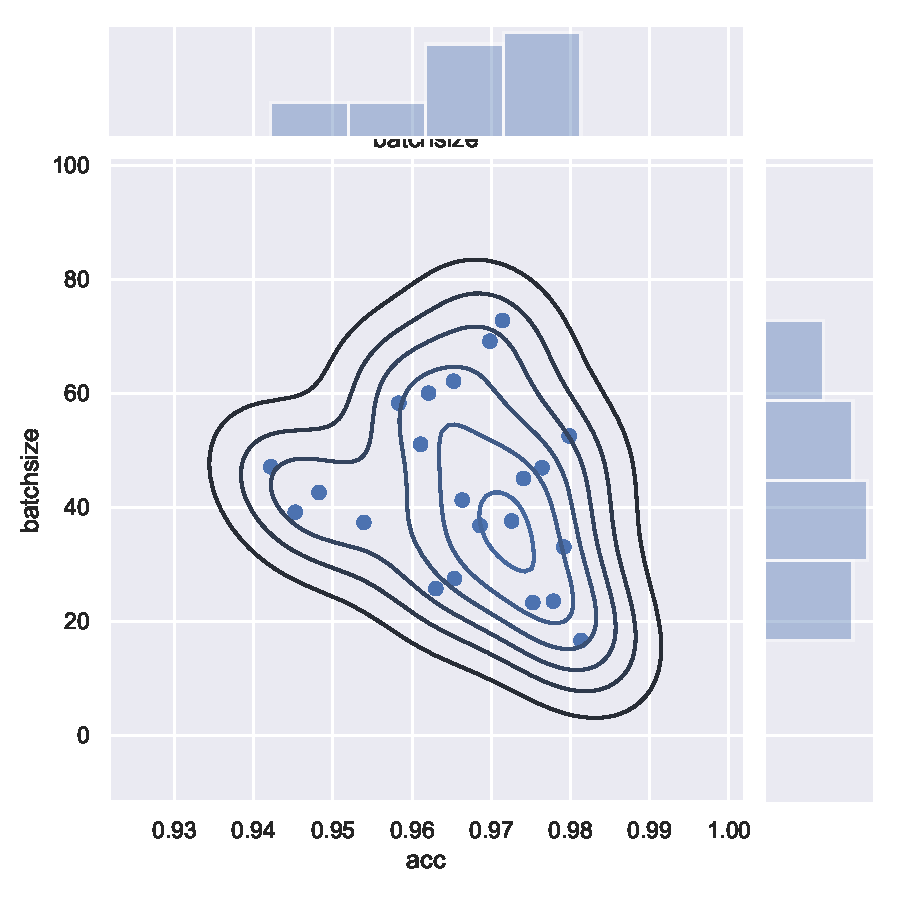
\includegraphics[scale=0.5]{anhang/GA_50_mnist_digits_False_small_jointplot_batchsize.pdf}
  \caption{Dichte-Diagramm der Batchsize in Verbindung mit der Klassifizierungsgenauigkeit(acc)}
  
\end{figure}

\begin{figure}[H]
  \centering  
  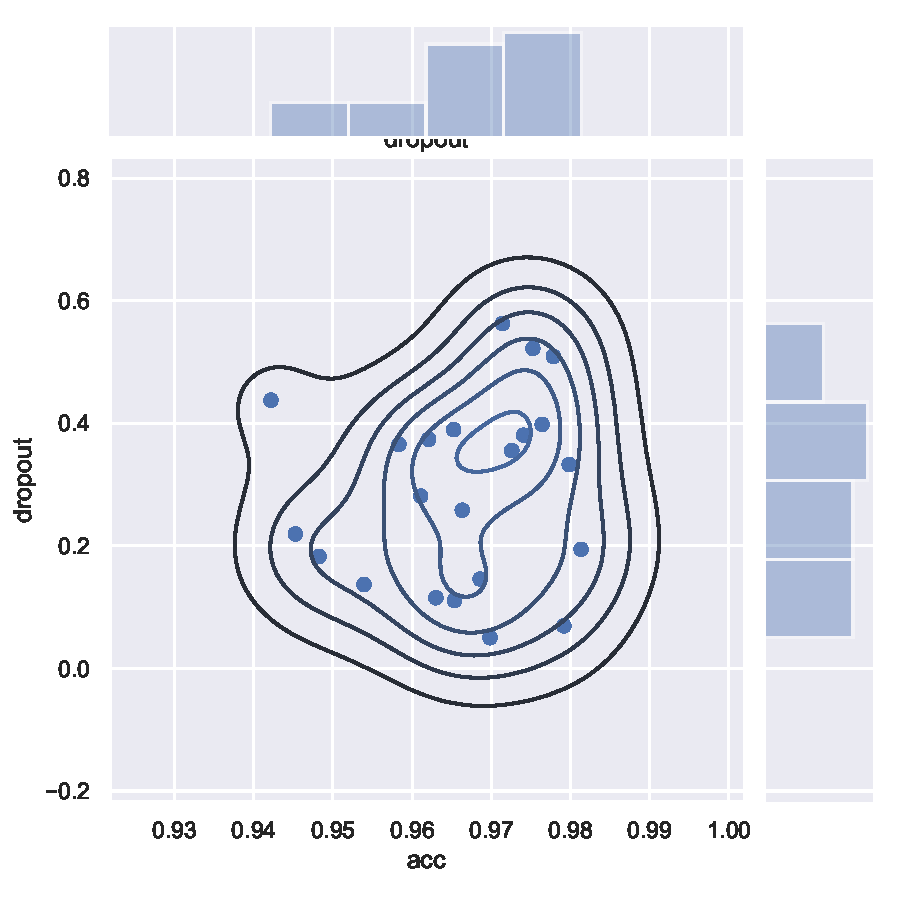
\includegraphics[scale=0.5]{anhang/GA_50_mnist_digits_False_small_jointplot_dropout.pdf}
  \caption{Dichte-Diagramm des Dropouts in Verbindung mit der Klassifizierungsgenauigkeit(acc)}
  
\end{figure}

\begin{figure}[H]
  \centering  
  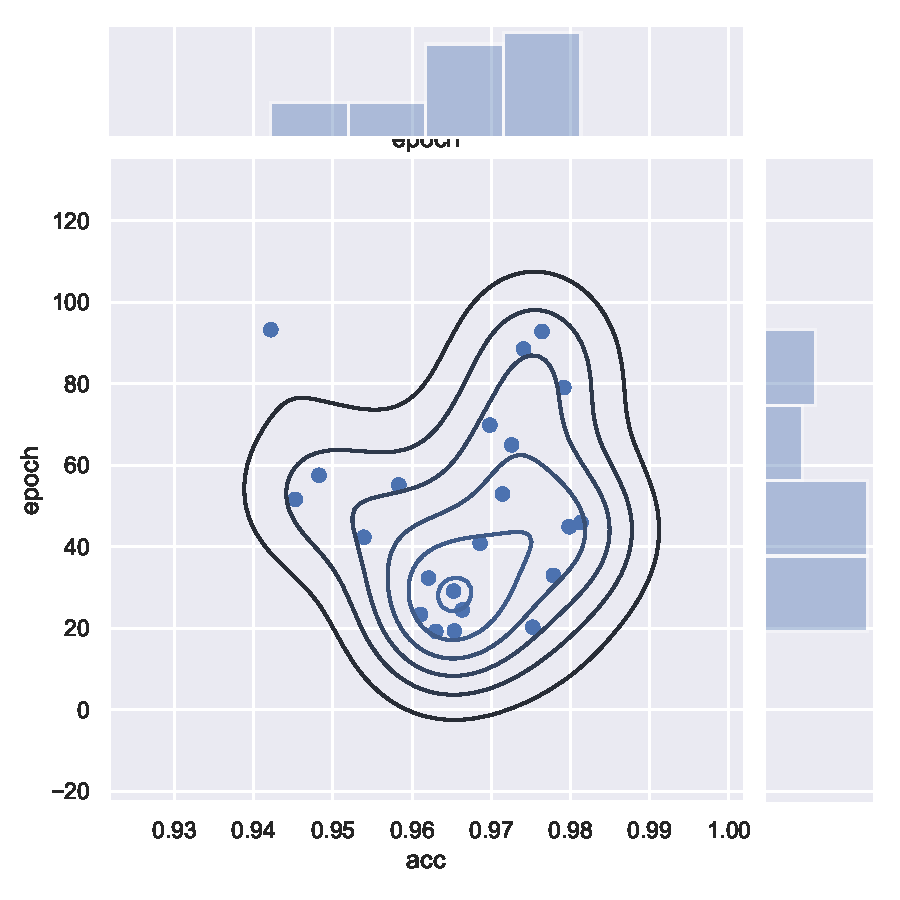
\includegraphics[scale=0.5]{anhang/GA_50_mnist_digits_False_small_jointplot_epoch.pdf}
  \caption{Dichte-Diagramm der Epochenanzahl in Verbindung mit der Klassifizierungsgenauigkeit(acc)}
  
\end{figure}

\begin{figure}[H]
  \centering  
  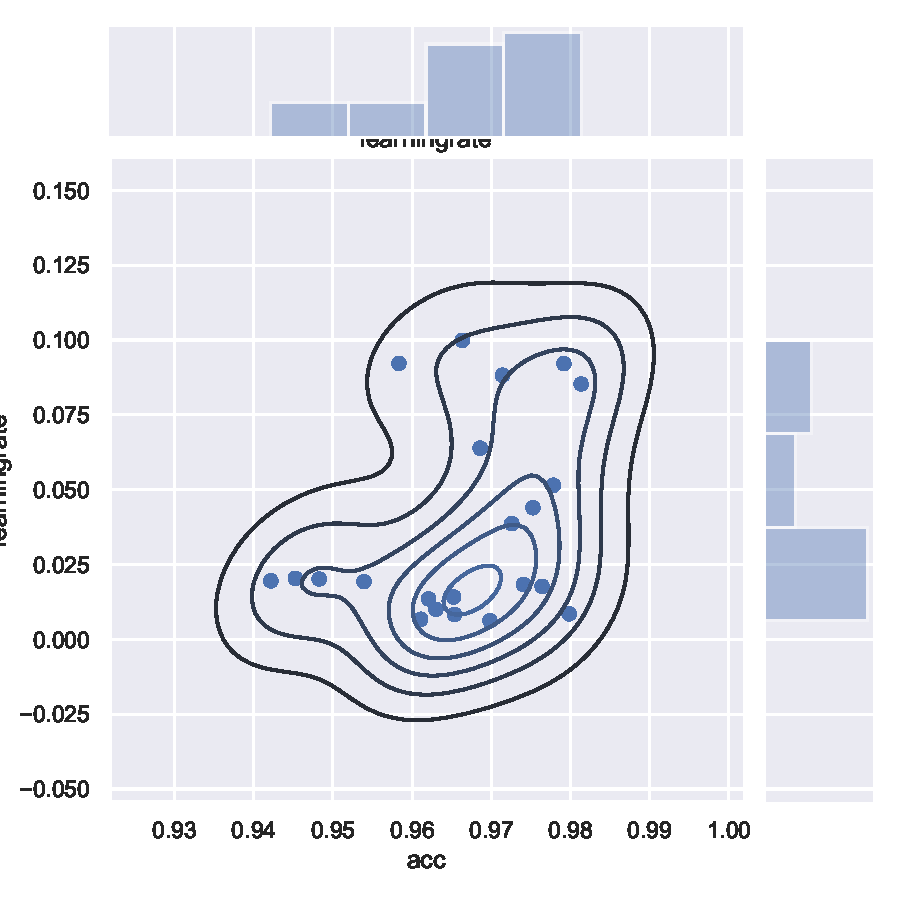
\includegraphics[scale=0.5]{anhang/GA_50_mnist_digits_False_small_jointplot_learningrate.pdf}
  \caption{Dichte-Diagramm der Lernrate in Verbindung mit der Klassifizierungsgenauigkeit(acc)}
  
\end{figure}

\begin{figure}[H]
  \centering  
  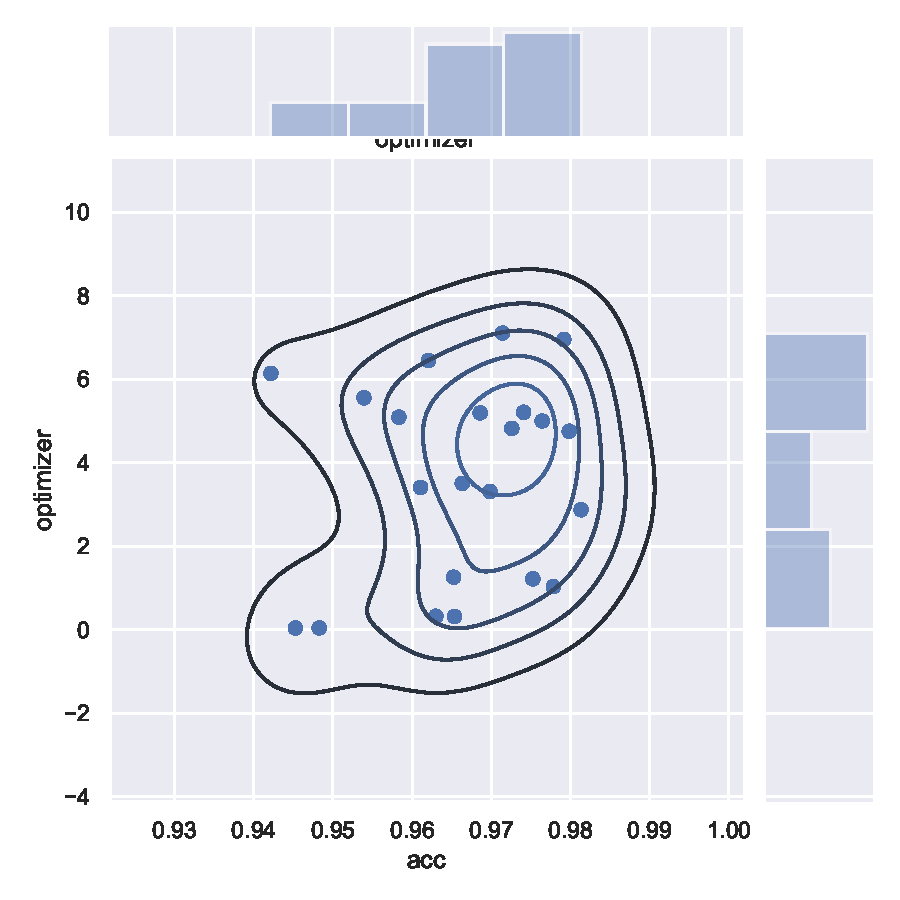
\includegraphics[scale=0.5]{anhang/GA_50_mnist_digits_False_small_jointplot_optimizer.pdf}
  \caption{Dichte-Diagramm des Optimierers in Verbindung mit der Klassifizierungsgenauigkeit(acc)}
  
\end{figure}

\subsection{50 Iterationen des Genetischen Algorithmus des großen Fully-Connected Netzes}
\begin{figure}[H]
  \centering  
  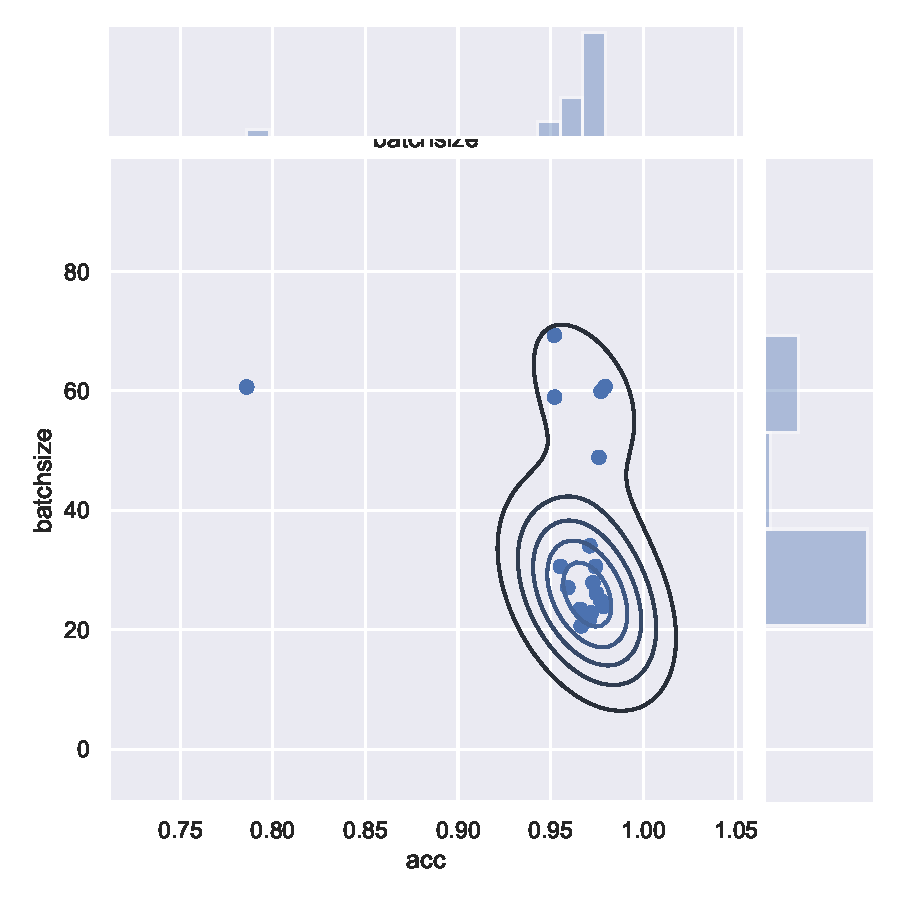
\includegraphics[scale=0.5]{anhang/GA_50_mnist_digits_False_big_jointplot_batchsize.pdf}
  \caption{Dichte-Diagramm der Batchsize in Verbindung mit der Klassifizierungsgenauigkeit(acc)}
  
\end{figure}

\begin{figure}[H]
  \centering  
  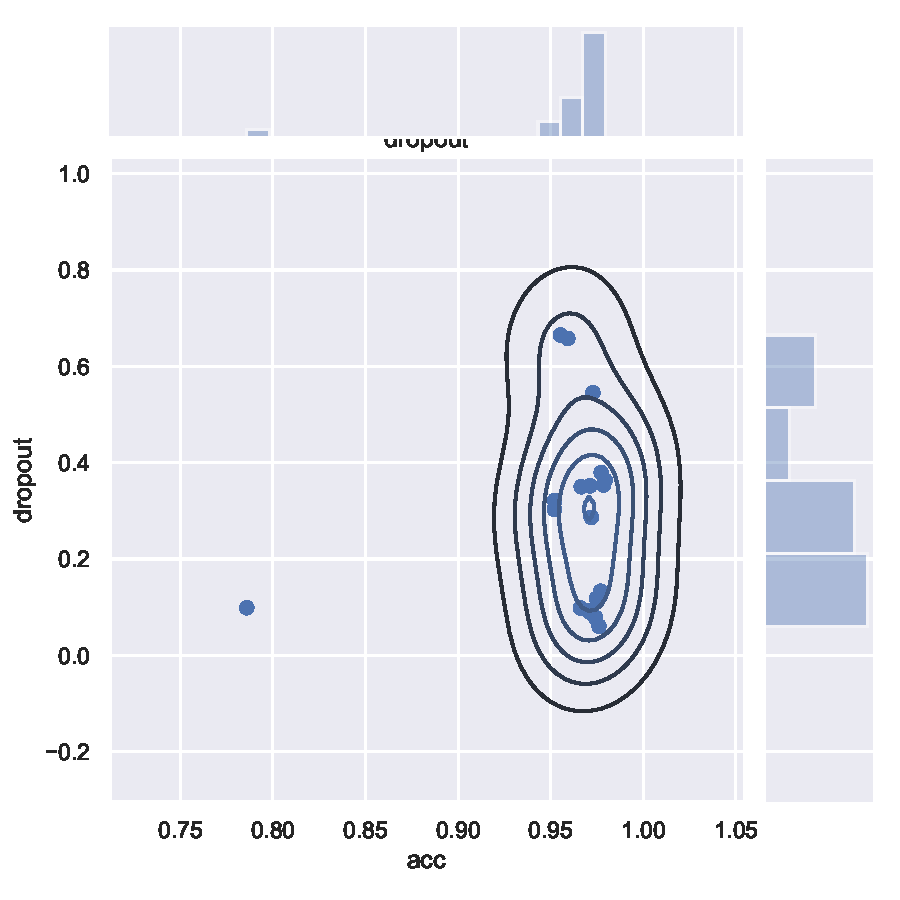
\includegraphics[scale=0.5]{anhang/GA_50_mnist_digits_False_big_jointplot_dropout.pdf}
  \caption{Dichte-Diagramm des Dropouts in Verbindung mit der Klassifizierungsgenauigkeit(acc)}
  
\end{figure}

\begin{figure}[H]
  \centering  
  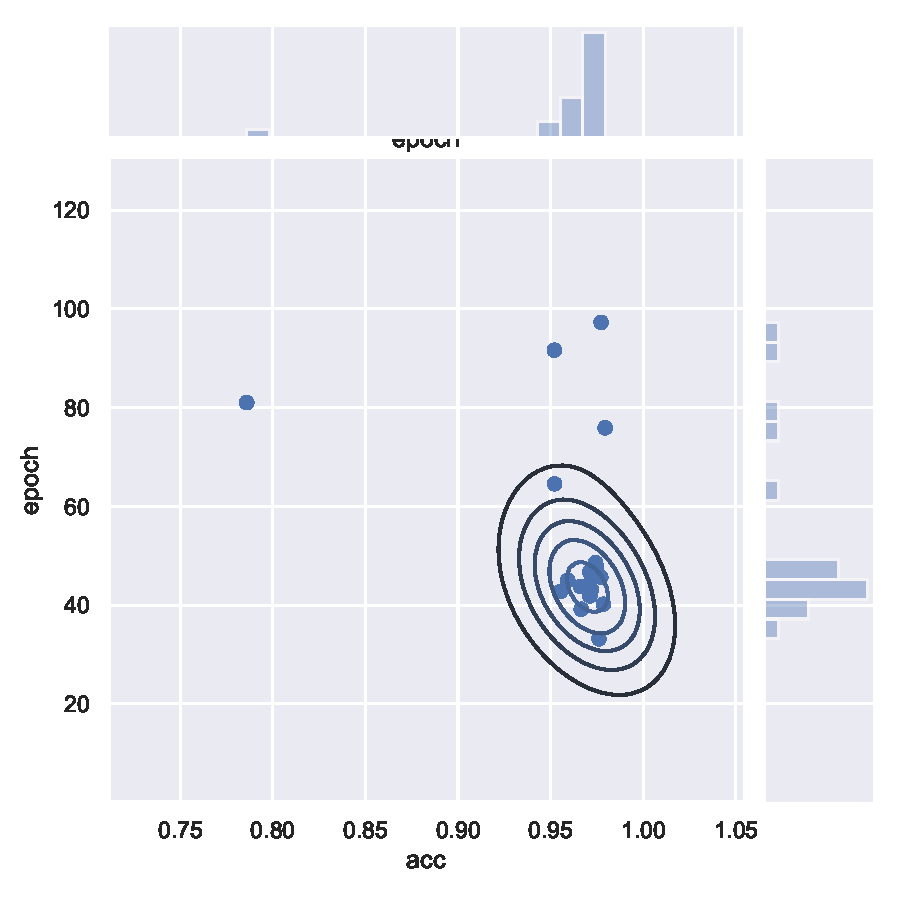
\includegraphics[scale=0.5]{anhang/GA_50_mnist_digits_False_big_jointplot_epoch.pdf}
  \caption{Dichte-Diagramm der Epochenanzahl in Verbindung mit der Klassifizierungsgenauigkeit(acc)}
  
\end{figure}

\begin{figure}[H]
  \centering  
  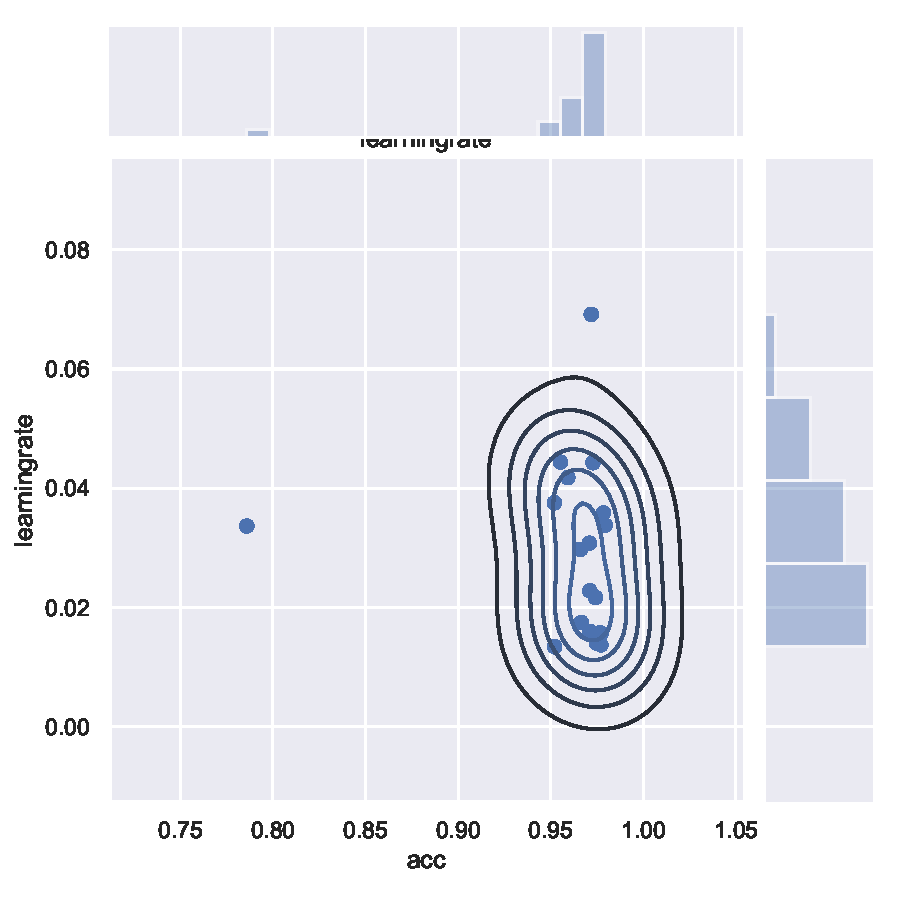
\includegraphics[scale=0.5]{anhang/GA_50_mnist_digits_False_big_jointplot_learningrate.pdf}
  \caption{Dichte-Diagramm der Lernrate in Verbindung mit der Klassifizierungsgenauigkeit(acc)}
  
\end{figure}

\begin{figure}[H]
  \centering  
  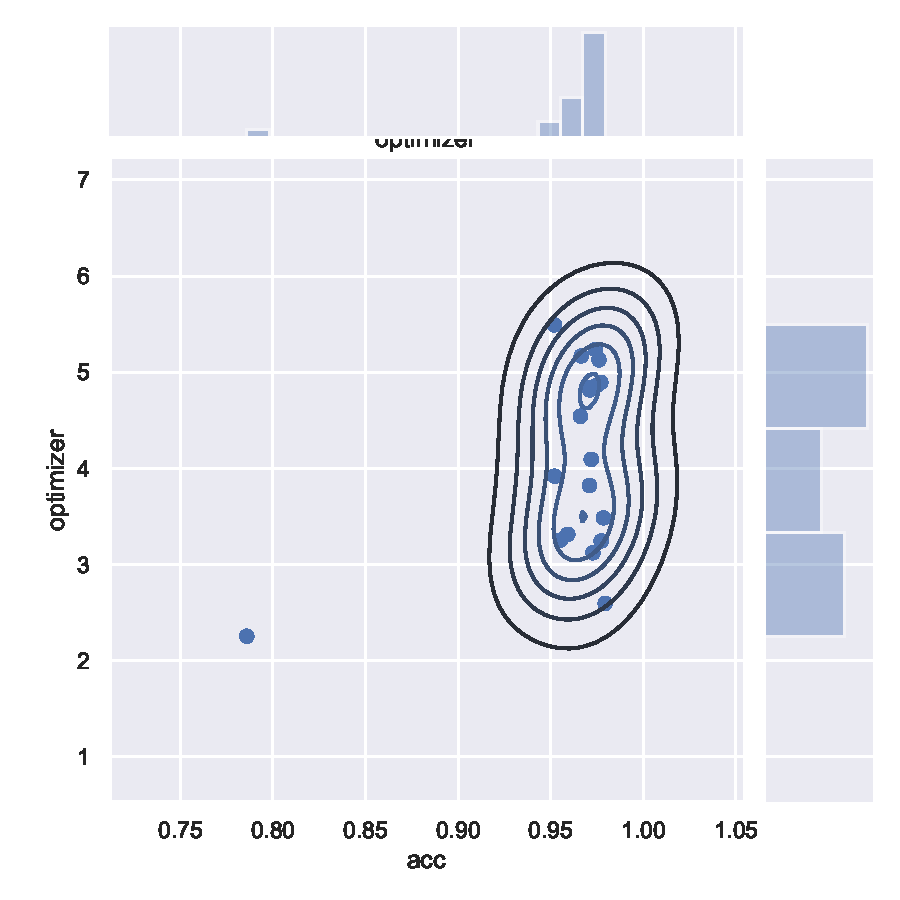
\includegraphics[scale=0.5]{anhang/GA_50_mnist_digits_False_big_jointplot_optimizer.pdf}
  \caption{Dichte-Diagramm des Optimierers in Verbindung mit der Klassifizierungsgenauigkeit(acc)}
  
\end{figure}


\subsection{250 Iterationen des Genetischen Algorithmus des kleinen Fully-Connected Netzes}
\begin{figure}[H]
  \centering  
  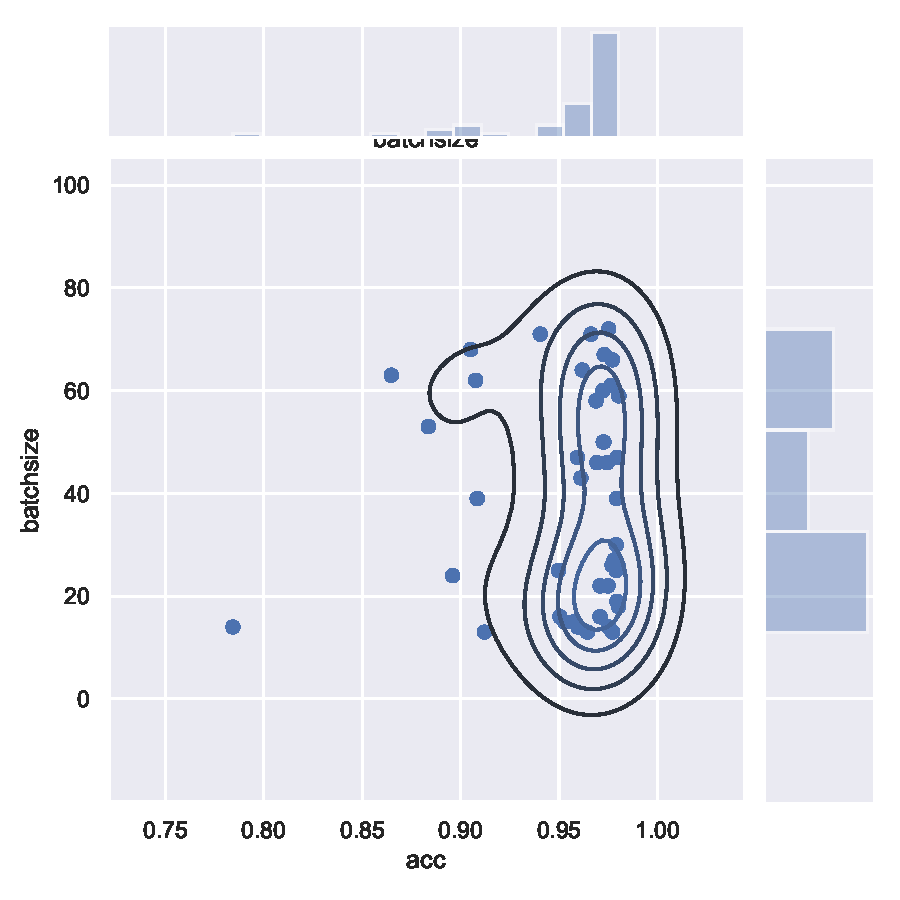
\includegraphics[scale=0.5]{anhang/GA_250_mnist_digits_False_small_jointplot_batchsize.pdf}
  \caption{Dichte-Diagramm der Batchsize in Verbindung mit der Klassifizierungsgenauigkeit(acc)}
  
\end{figure}

\begin{figure}[H]
  \centering  
  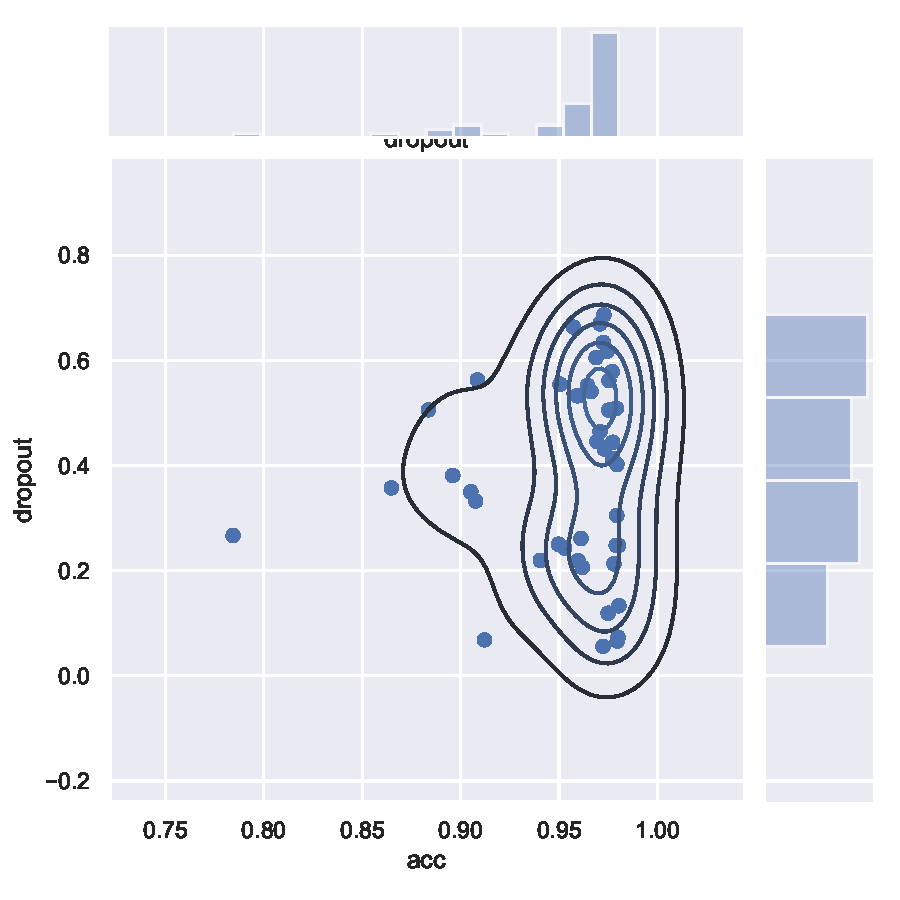
\includegraphics[scale=0.5]{anhang/GA_250_mnist_digits_False_small_jointplot_dropout.pdf}
  \caption{Dichte-Diagramm des Dropouts in Verbindung mit der Klassifizierungsgenauigkeit(acc)}
  
\end{figure}

\begin{figure}[H]
  \centering  
  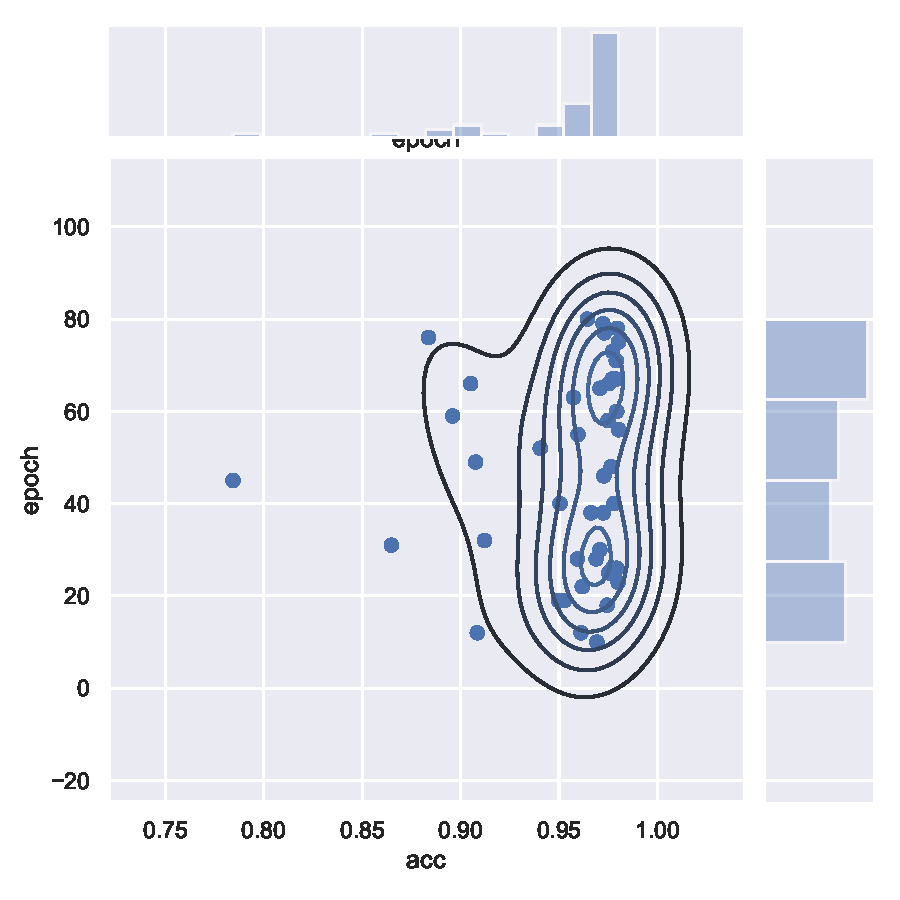
\includegraphics[scale=0.5]{anhang/GA_250_mnist_digits_False_small_jointplot_epoch.pdf}
  \caption{Dichte-Diagramm der Epochenanzahl in Verbindung mit der Klassifizierungsgenauigkeit(acc)}
  
\end{figure}

\begin{figure}[H]
  \centering  
  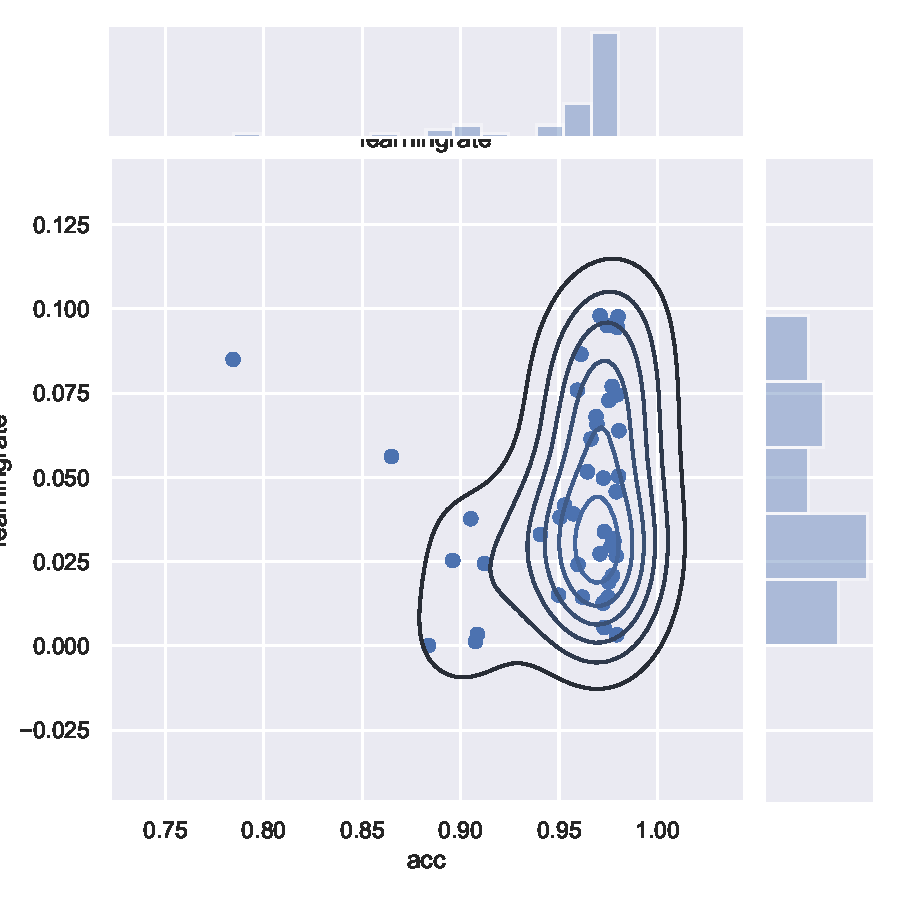
\includegraphics[scale=0.5]{anhang/GA_250_mnist_digits_False_small_jointplot_learningrate.pdf}
  \caption{Dichte-Diagramm der Lernrate in Verbindung mit der Klassifizierungsgenauigkeit(acc)}
  
\end{figure}

\begin{figure}[H]
  \centering  
  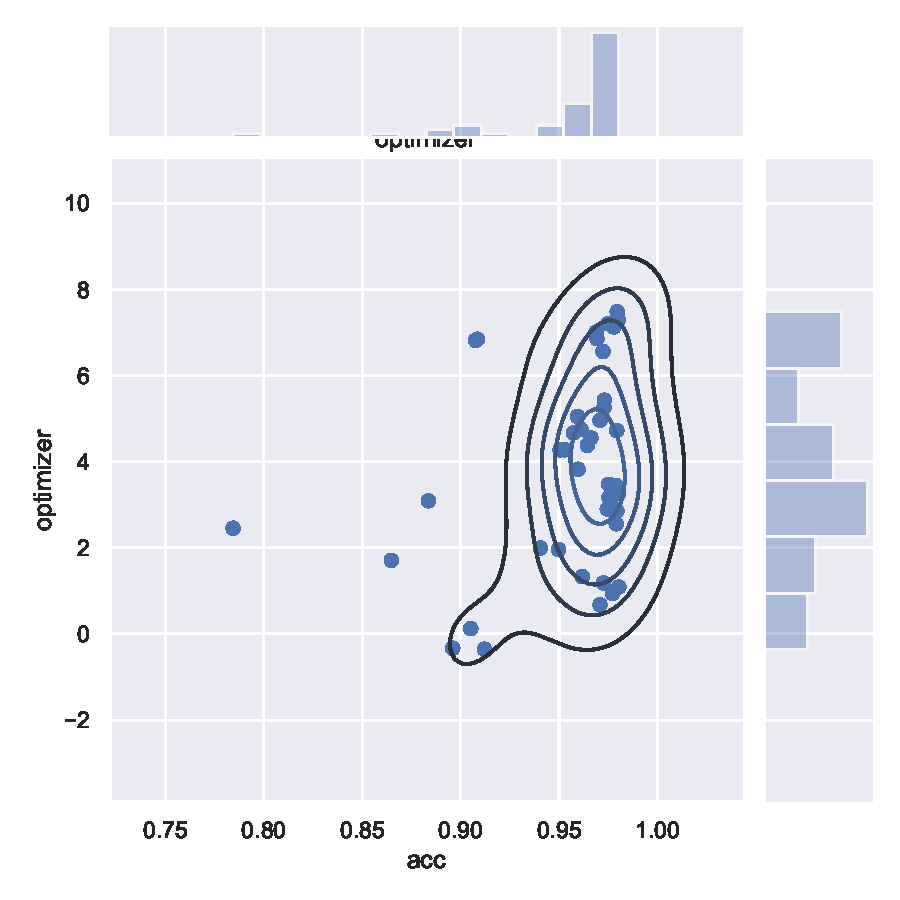
\includegraphics[scale=0.5]{anhang/GA_250_mnist_digits_False_small_jointplot_optimizer.pdf}
  \caption{Dichte-Diagramm des Optimierers in Verbindung mit der Klassifizierungsgenauigkeit(acc)}
  
\end{figure}

\subsection{250 Iterationen des Genetischen Algorithmus des großen Fully-Connected Netzes}
\begin{figure}[H]
  \centering  
  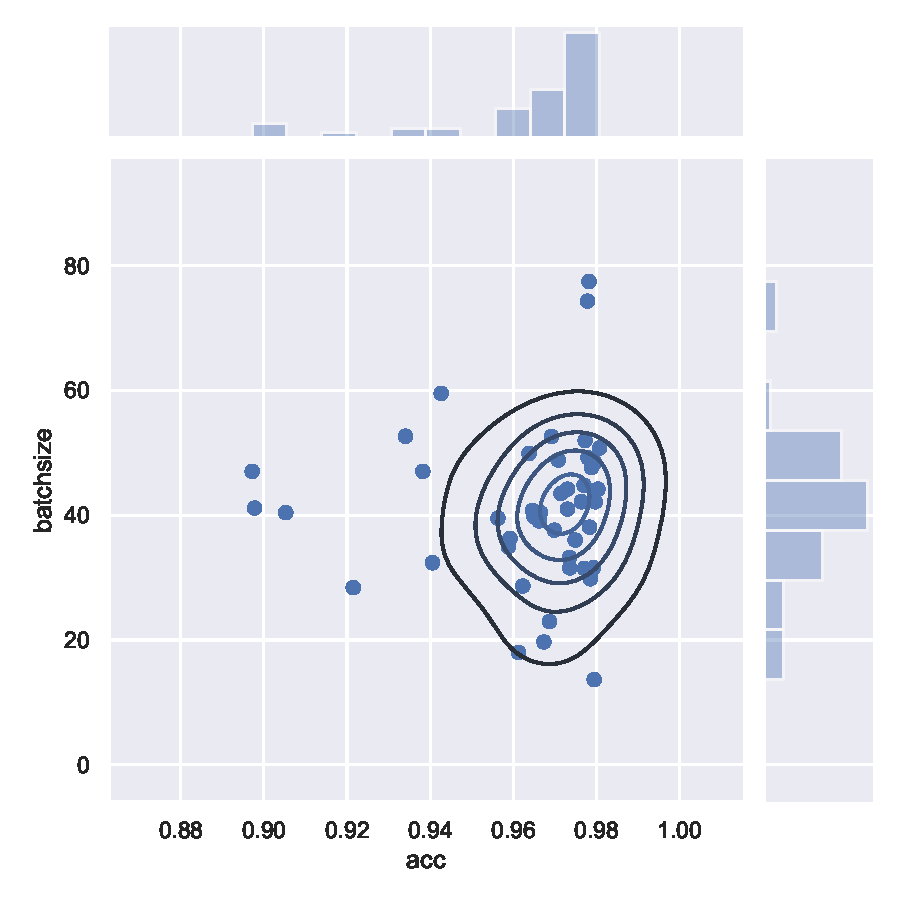
\includegraphics[scale=0.5]{anhang/GA_250_mnist_digits_False_big_jointplot_batchsize.pdf}
  \caption{Dichte-Diagramm der Batchsize in Verbindung mit der Klassifizierungsgenauigkeit(acc)}
  
\end{figure}

\begin{figure}[H]
  \centering  
  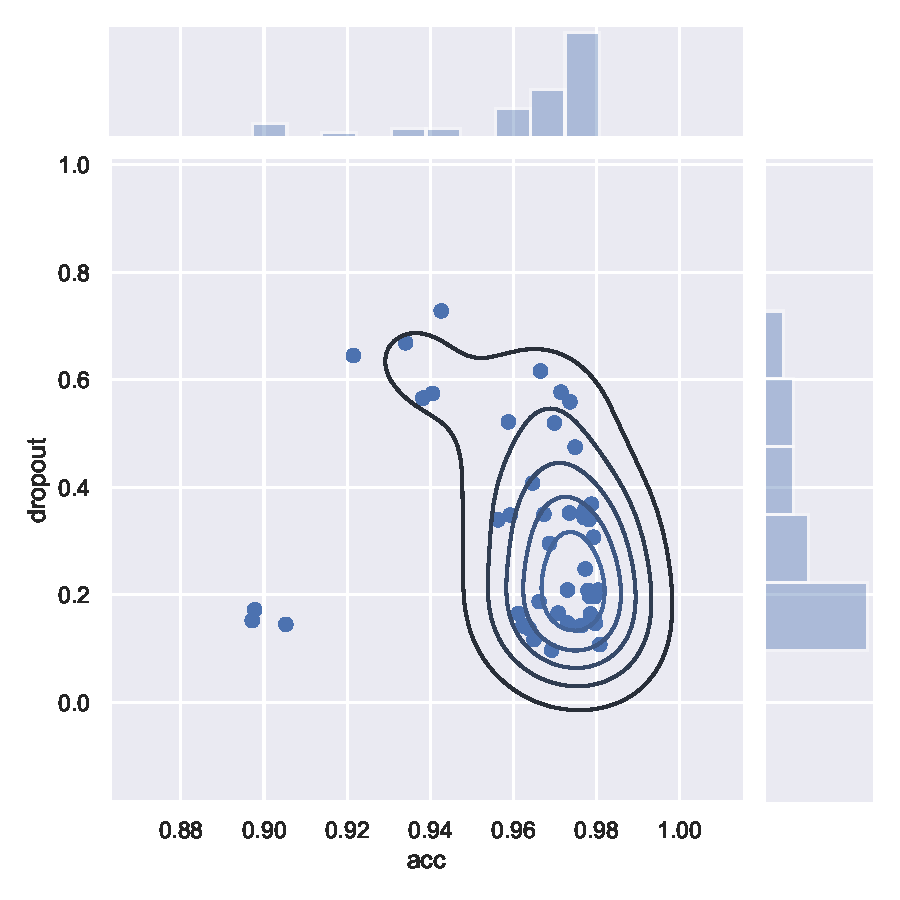
\includegraphics[scale=0.5]{anhang/GA_250_mnist_digits_False_big_jointplot_dropout.pdf}
  \caption{Dichte-Diagramm des Dropouts in Verbindung mit der Klassifizierungsgenauigkeit(acc)}
  
\end{figure}

\begin{figure}[H]
  \centering  
  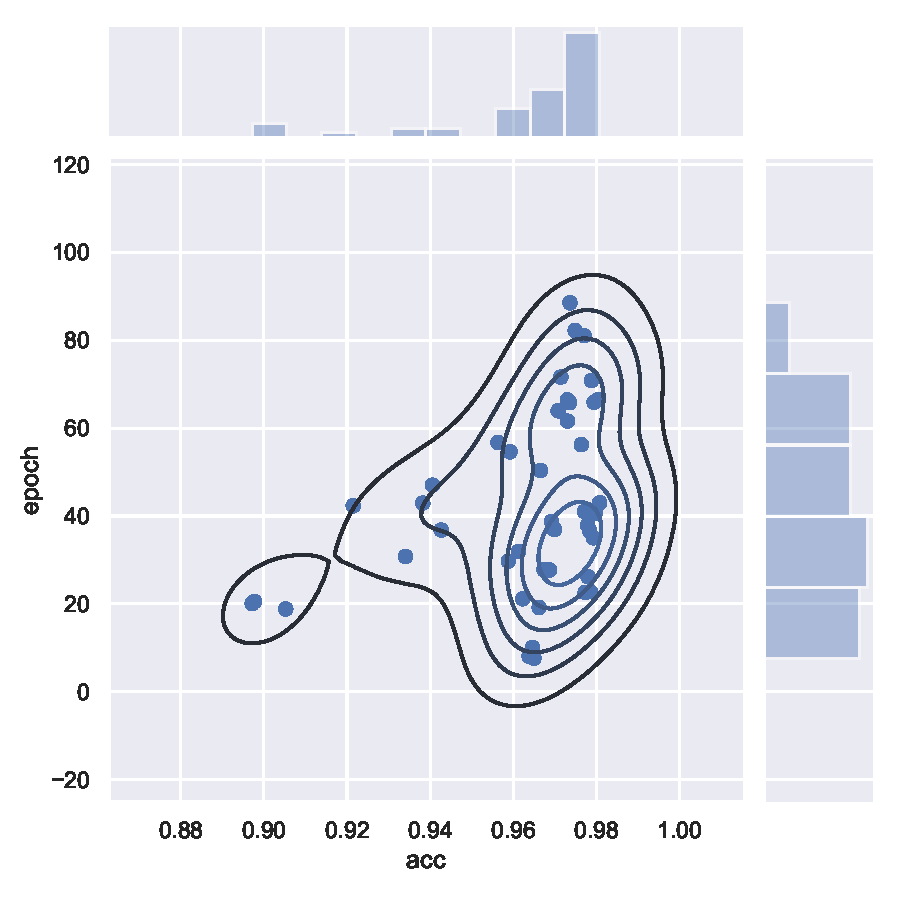
\includegraphics[scale=0.5]{anhang/GA_250_mnist_digits_False_big_jointplot_epoch.pdf}
  \caption{Dichte-Diagramm der Epochenanzahl in Verbindung mit der Klassifizierungsgenauigkeit(acc)}
  
\end{figure}

\begin{figure}[H]
  \centering  
  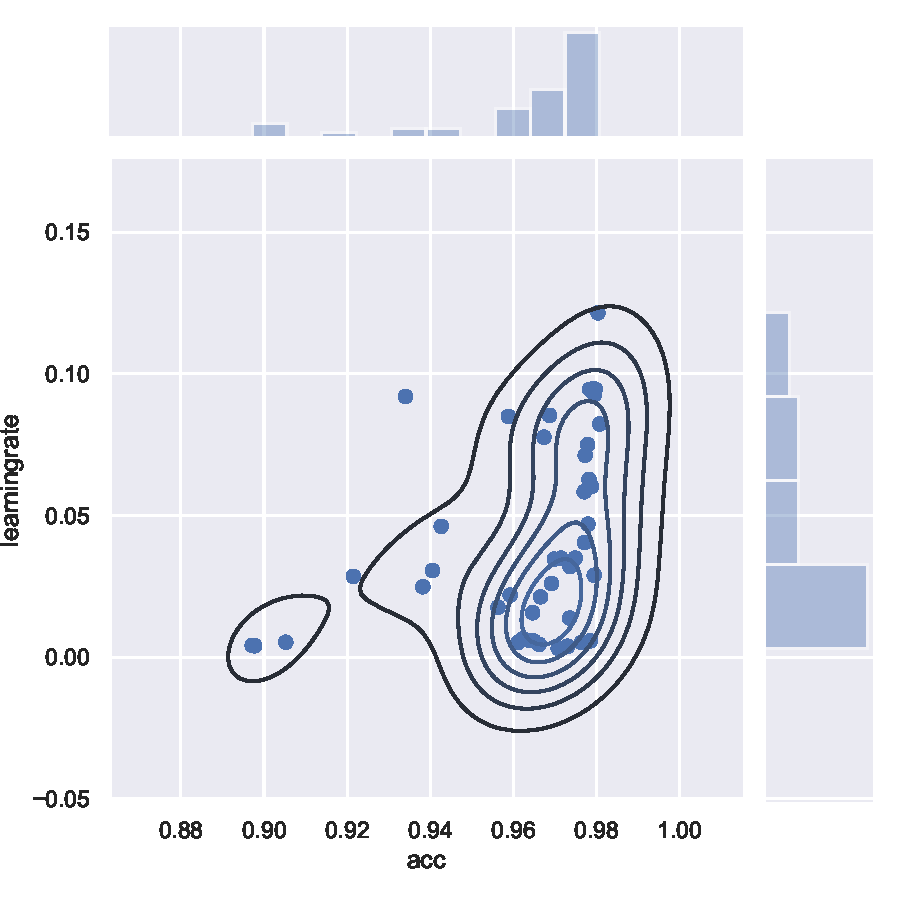
\includegraphics[scale=0.5]{anhang/GA_250_mnist_digits_False_big_jointplot_learningrate.pdf}
  \caption{Dichte-Diagramm der Lernrate in Verbindung mit der Klassifizierungsgenauigkeit(acc)}
  
\end{figure}

\begin{figure}[H]
  \centering  
  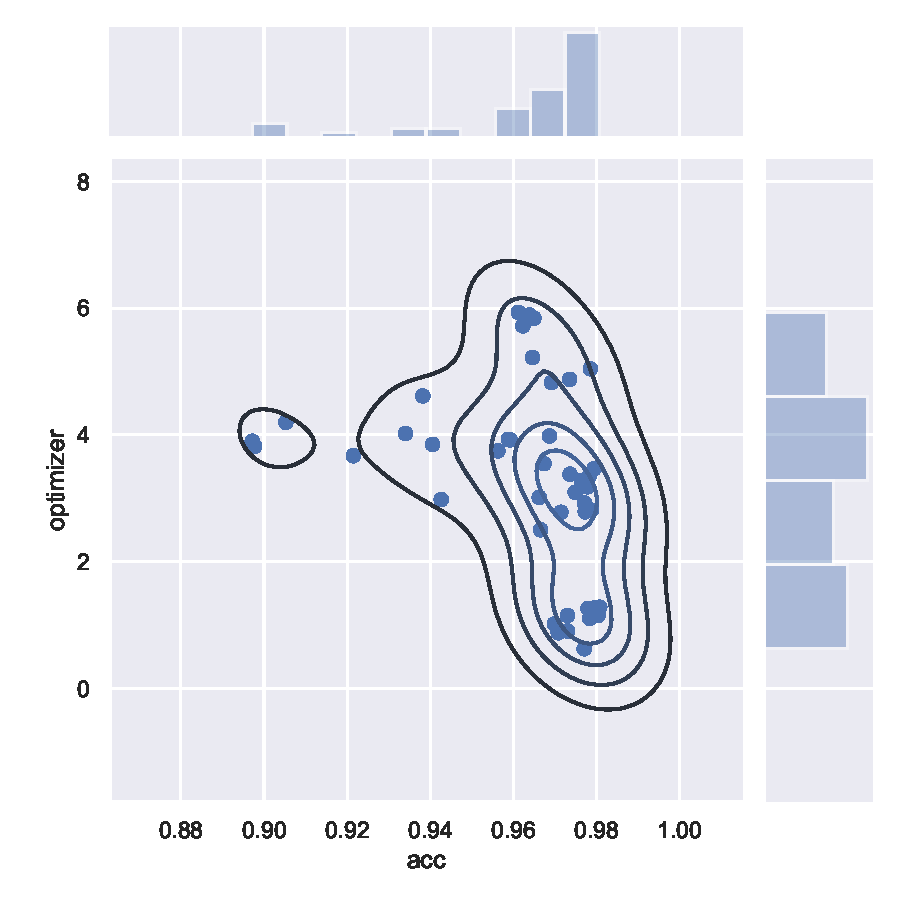
\includegraphics[scale=0.5]{anhang/GA_250_mnist_digits_False_big_jointplot_optimizer.pdf}
  \caption{Dichte-Diagramm des Optimierers in Verbindung mit der Klassifizierungsgenauigkeit(acc)}
  
\end{figure}

\subsection{50 Iterationen des Genetischen Algorithmus des Convolutional Neural Network}
\begin{figure}[H]
  \centering  
  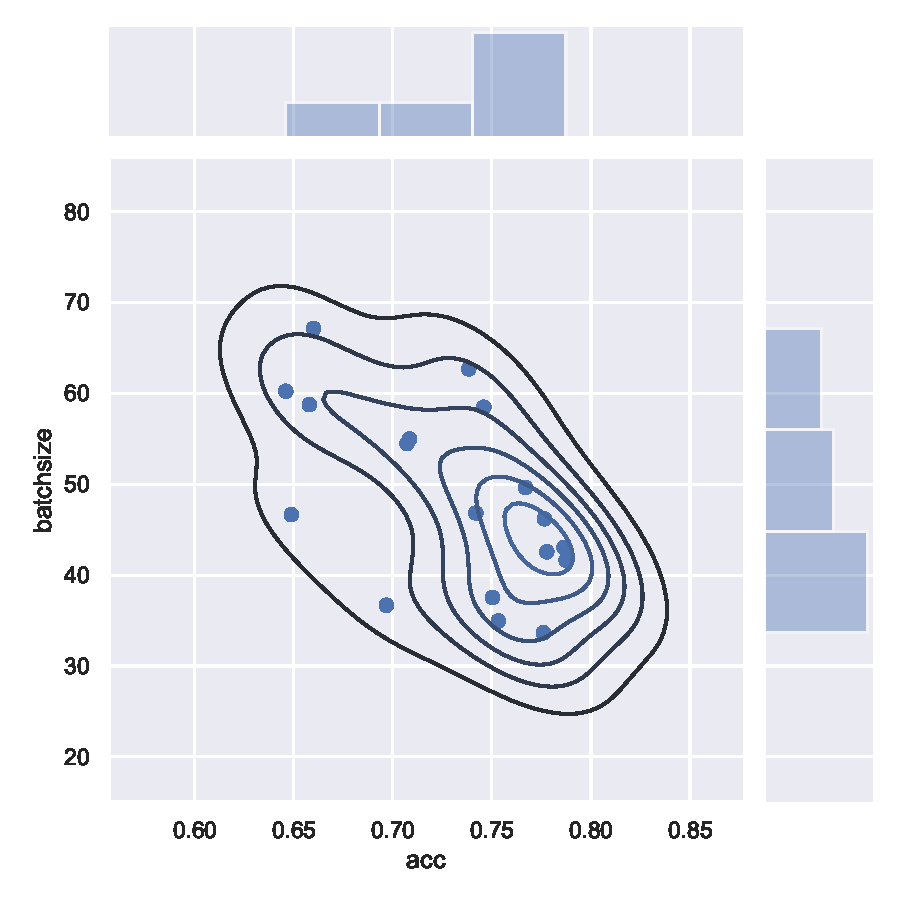
\includegraphics[scale=0.5]{anhang/GA_50_cifar10_False_big_jointplot_batchsize.pdf}
  \caption{Dichte-Diagramm der Batchsize in Verbindung mit der Klassifizierungsgenauigkeit(acc)}
  
\end{figure}

\begin{figure}[H]
  \centering  
  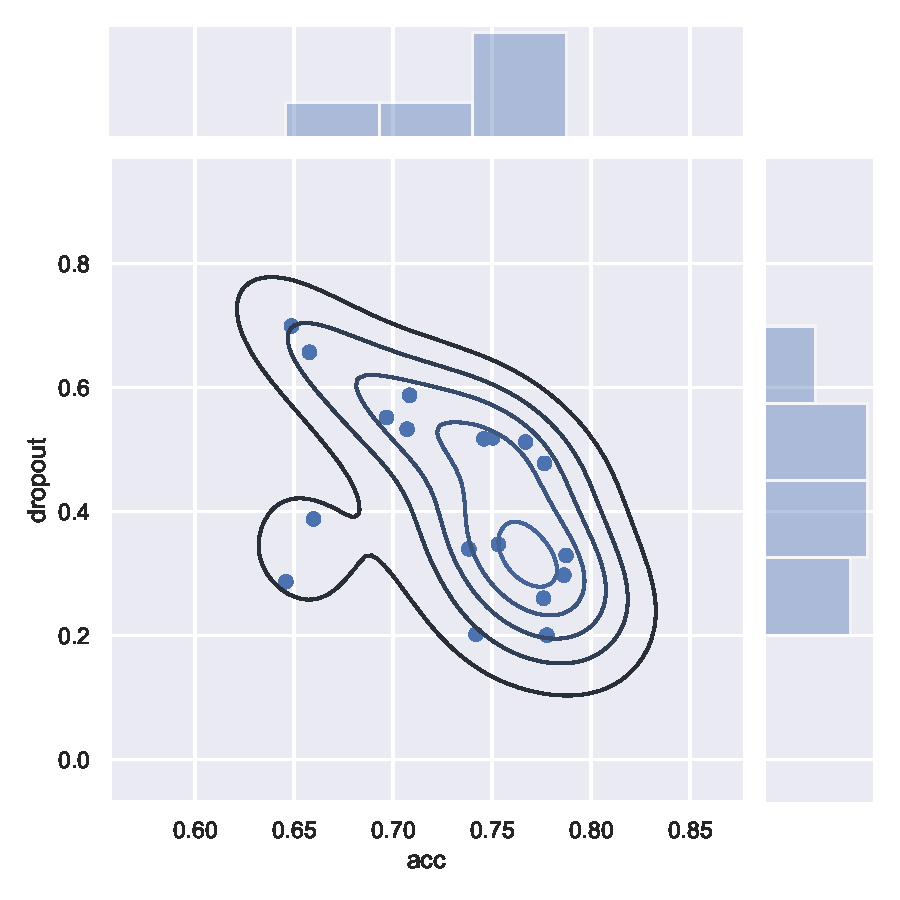
\includegraphics[scale=0.5]{anhang/GA_50_cifar10_False_big_jointplot_dropout.pdf}
  \caption{Dichte-Diagramm des Dropouts in Verbindung mit der Klassifizierungsgenauigkeit(acc)}
  
\end{figure}

\begin{figure}[H]
  \centering  
  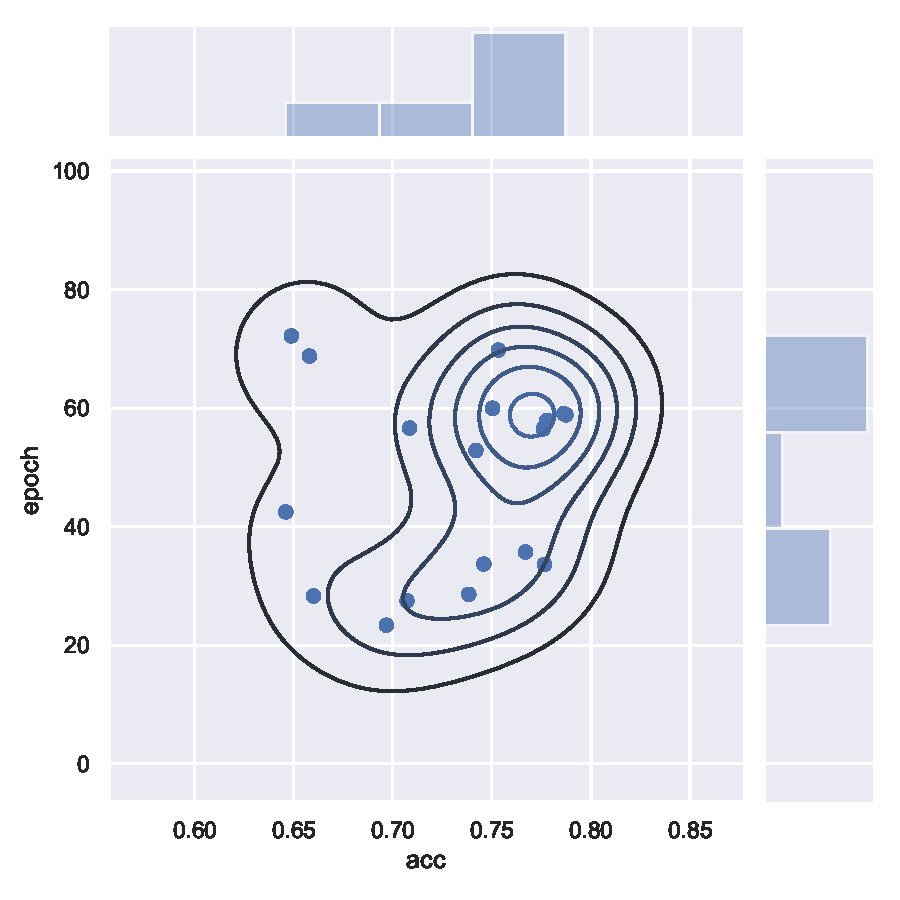
\includegraphics[scale=0.5]{anhang/GA_50_cifar10_False_big_jointplot_epoch.pdf}
  \caption{Dichte-Diagramm der Epochenanzahl in Verbindung mit der Klassifizierungsgenauigkeit(acc)}
  
\end{figure}

\begin{figure}[H]
  \centering  
  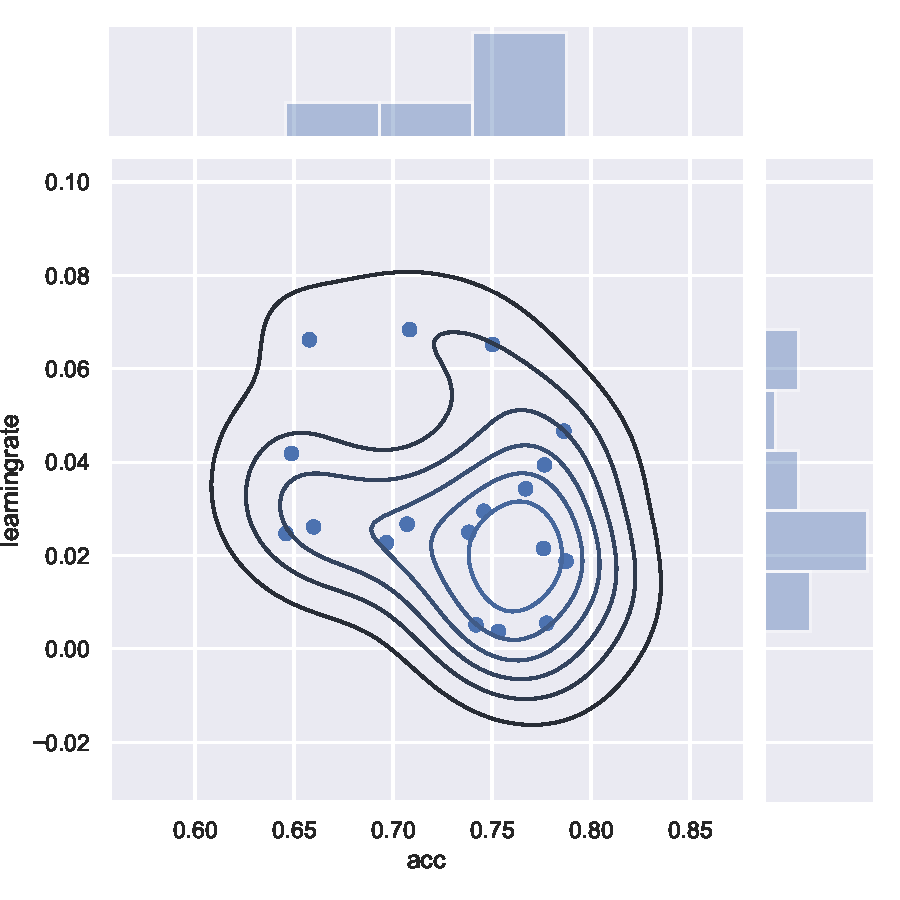
\includegraphics[scale=0.5]{anhang/GA_50_cifar10_False_big_jointplot_learningrate.pdf}
  \caption{Dichte-Diagramm der Lernrate in Verbindung mit der Klassifizierungsgenauigkeit(acc)}
  
\end{figure}

\begin{figure}[H]
  \centering  
  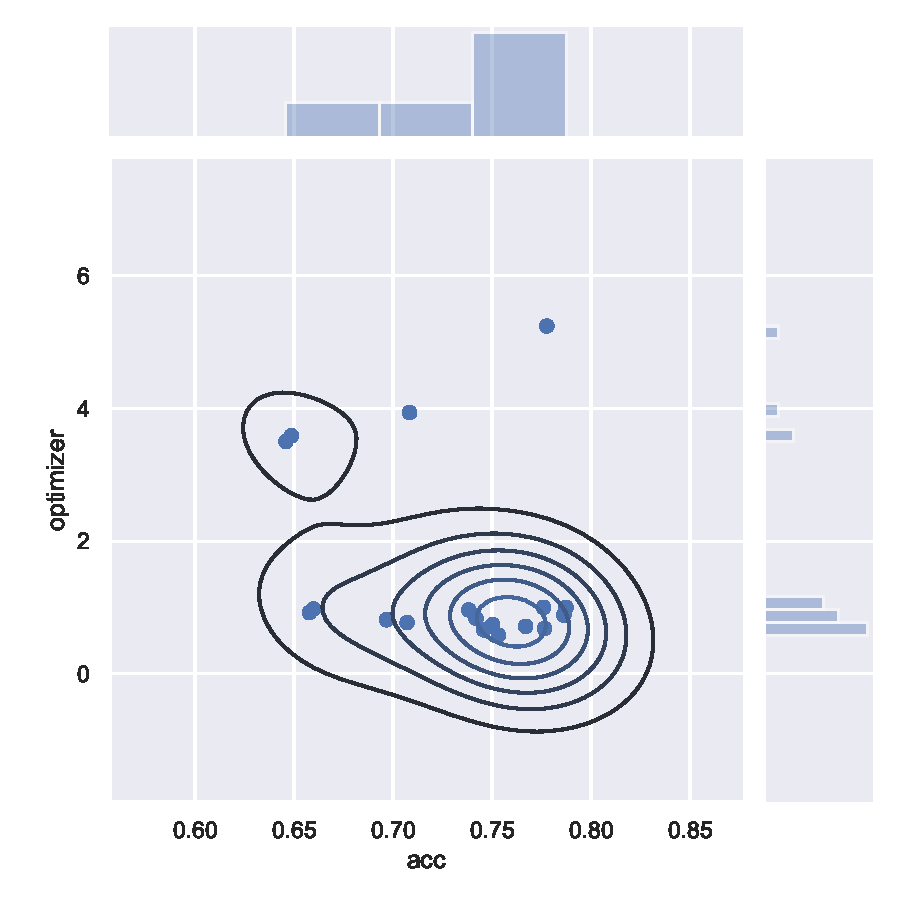
\includegraphics[scale=0.5]{anhang/GA_50_cifar10_False_big_jointplot_optimizer.pdf}
  \caption{Dichte-Diagramm des Optimierers in Verbindung mit der Klassifizierungsgenauigkeit(acc)}
\end{figure}

\subsection{250 Iterationen des Genetischen Algorithmus des Convolutional Neural Network}
\begin{figure}[H]
  \centering  
  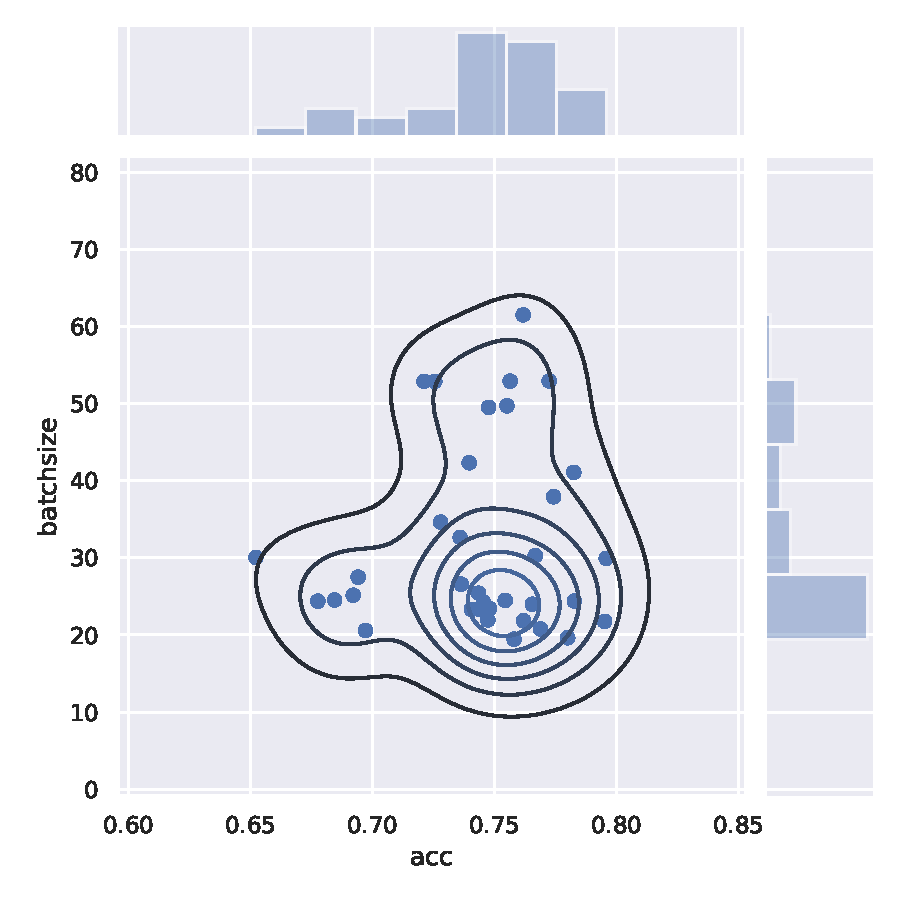
\includegraphics[scale=0.5]{anhang/GA_250_cifar10_False_big_jointplot_batchsize.pdf}
  \caption{Dichte-Diagramm der Batchsize in Verbindung mit der Klassifizierungsgenauigkeit(acc)}
\end{figure}

\begin{figure}[H]
  \centering  
  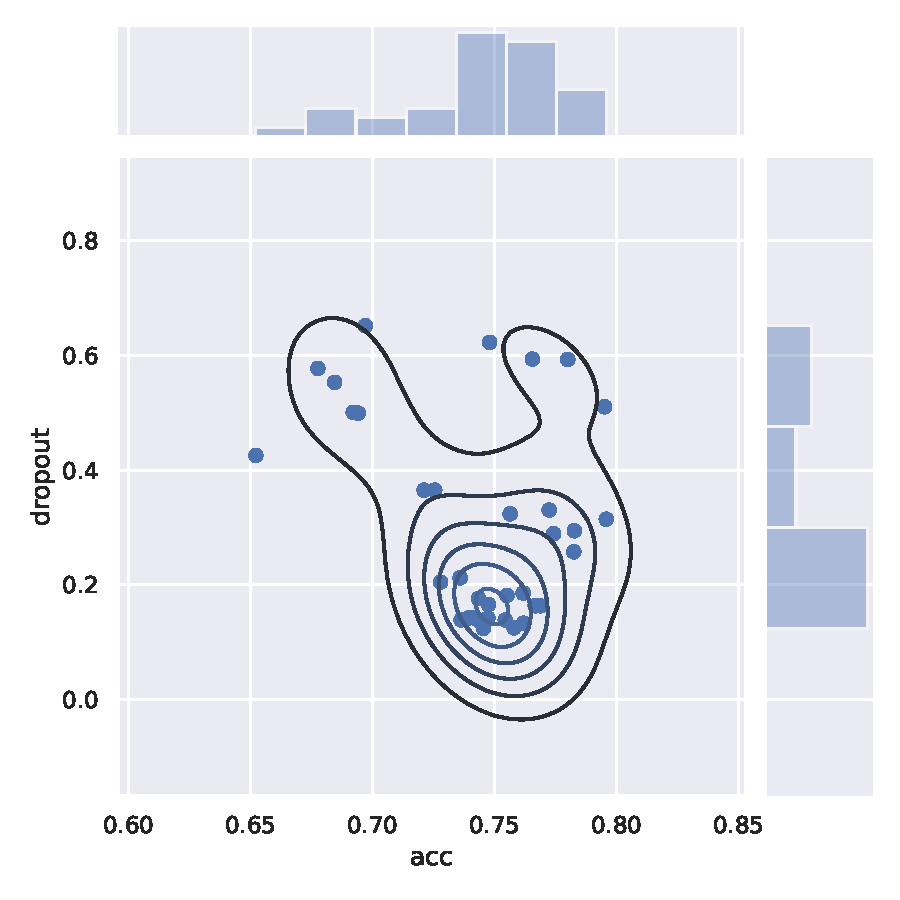
\includegraphics[scale=0.5]{anhang/GA_250_cifar10_False_big_jointplot_dropout.pdf}
  \caption{Dichte-Diagramm des Dropouts in Verbindung mit der Klassifizierungsgenauigkeit(acc)}
\end{figure}

\begin{figure}[H]
  \centering  
  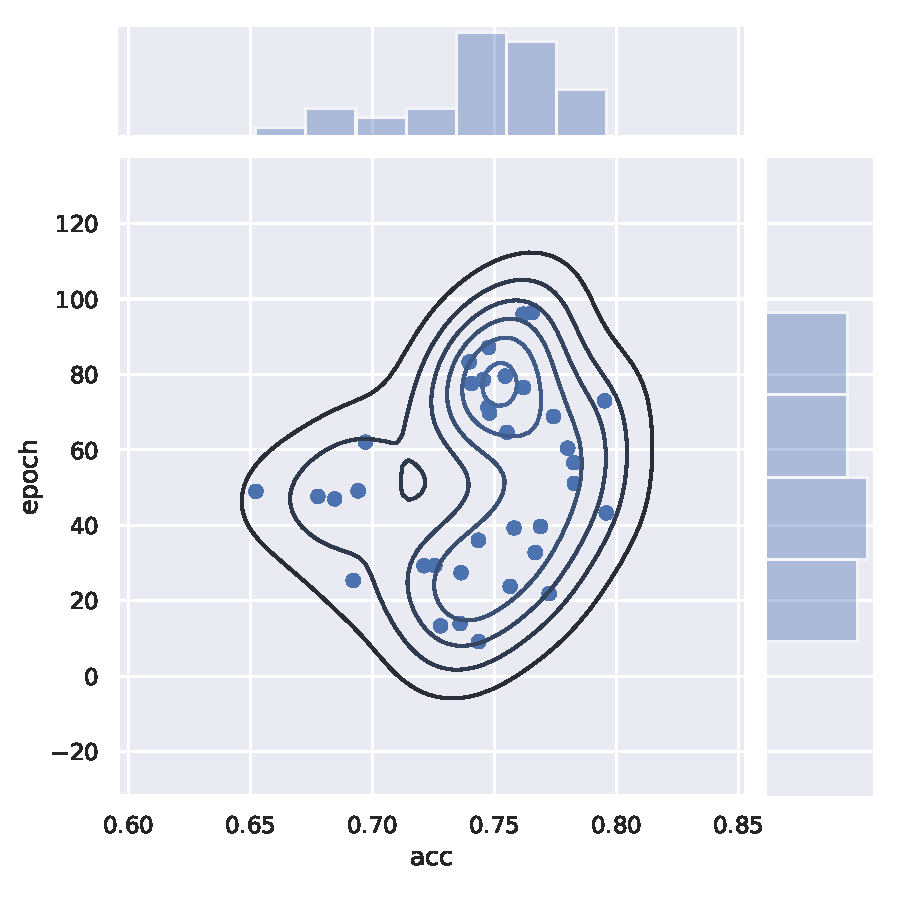
\includegraphics[scale=0.5]{anhang/GA_250_cifar10_False_big_jointplot_epoch.pdf}
  \caption{Dichte-Diagramm der Epochenanzahl in Verbindung mit der Klassifizierungsgenauigkeit(acc)}
\end{figure}

\begin{figure}[H]
  \centering  
  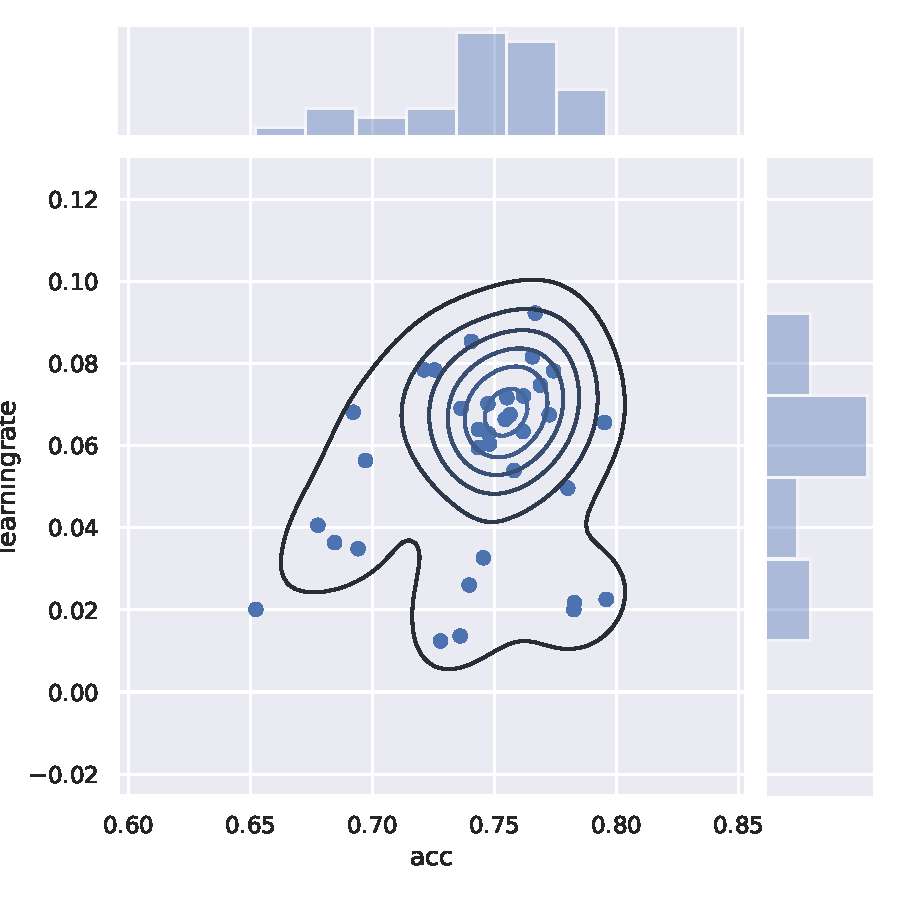
\includegraphics[scale=0.5]{anhang/GA_250_cifar10_False_big_jointplot_learningrate.pdf}
  \caption{Dichte-Diagramm der Lernrate in Verbindung mit der Klassifizierungsgenauigkeit(acc)}
\end{figure}

\begin{figure}[H]
  \centering  
  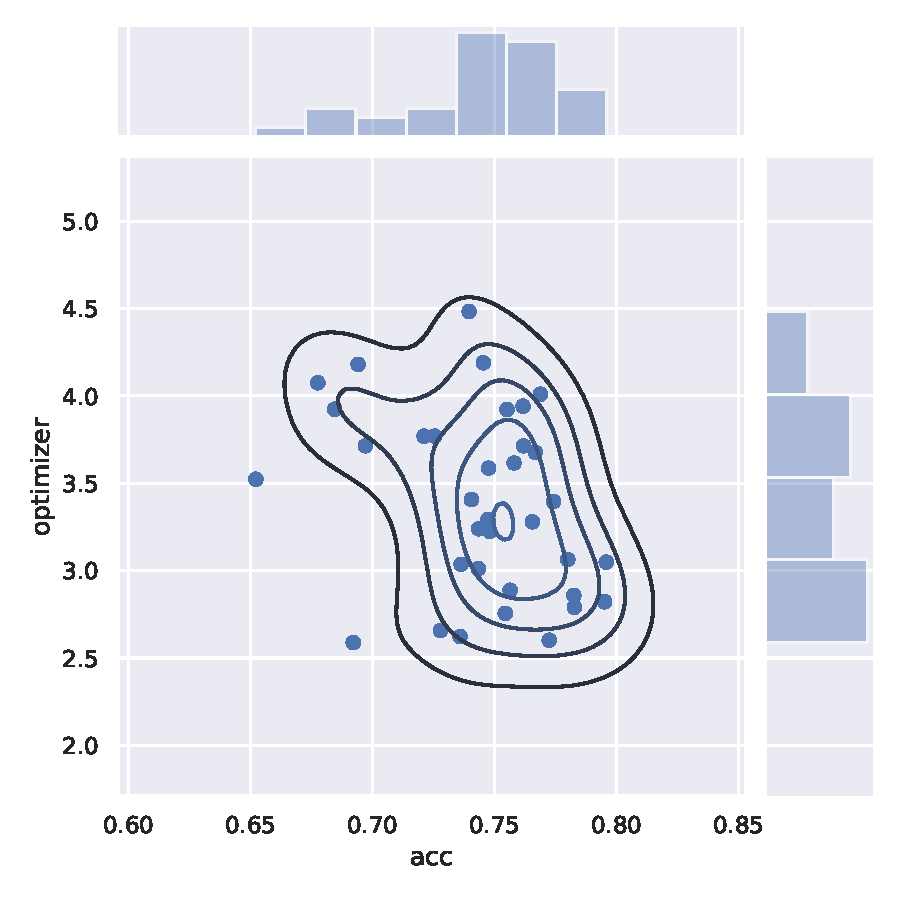
\includegraphics[scale=0.5]{anhang/GA_250_cifar10_False_big_jointplot_optimizer.pdf}
  \caption{Dichte-Diagramm des Optimierers in Verbindung mit der Klassifizierungsgenauigkeit(acc)}

\end{figure}



\section{Dichte-Diagramme zu den durchgeführten Optimierungen mit dem verkleinerten Datensatz}

\subsection{50 Iterationen des Genetischen Algorithmus des kleinen Fully-Connected Netzes}
\begin{figure}[H]
  \centering  
  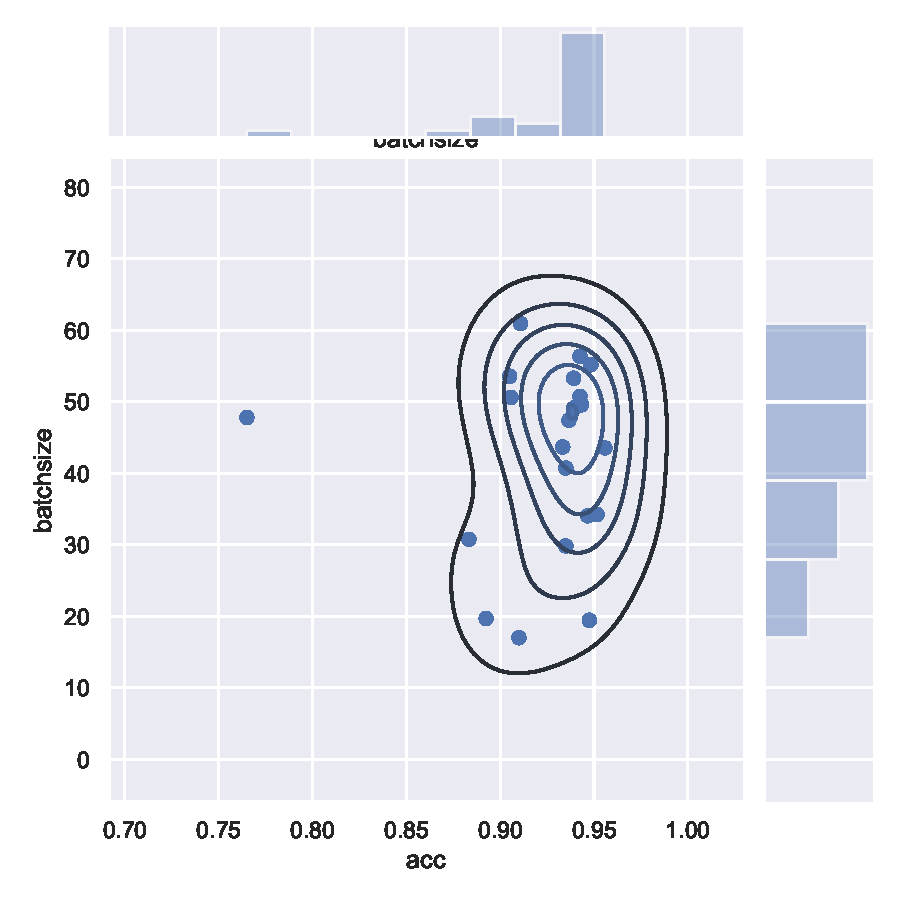
\includegraphics[scale=0.5]{anhang/GA_50_mnist_digits_True_small_jointplot_batchsize.pdf}
  \caption{Dichte-Diagramm der Batchsize in Verbindung mit der Klassifizierungsgenauigkeit(acc)}
  
\end{figure}

\begin{figure}[H]
  \centering  
  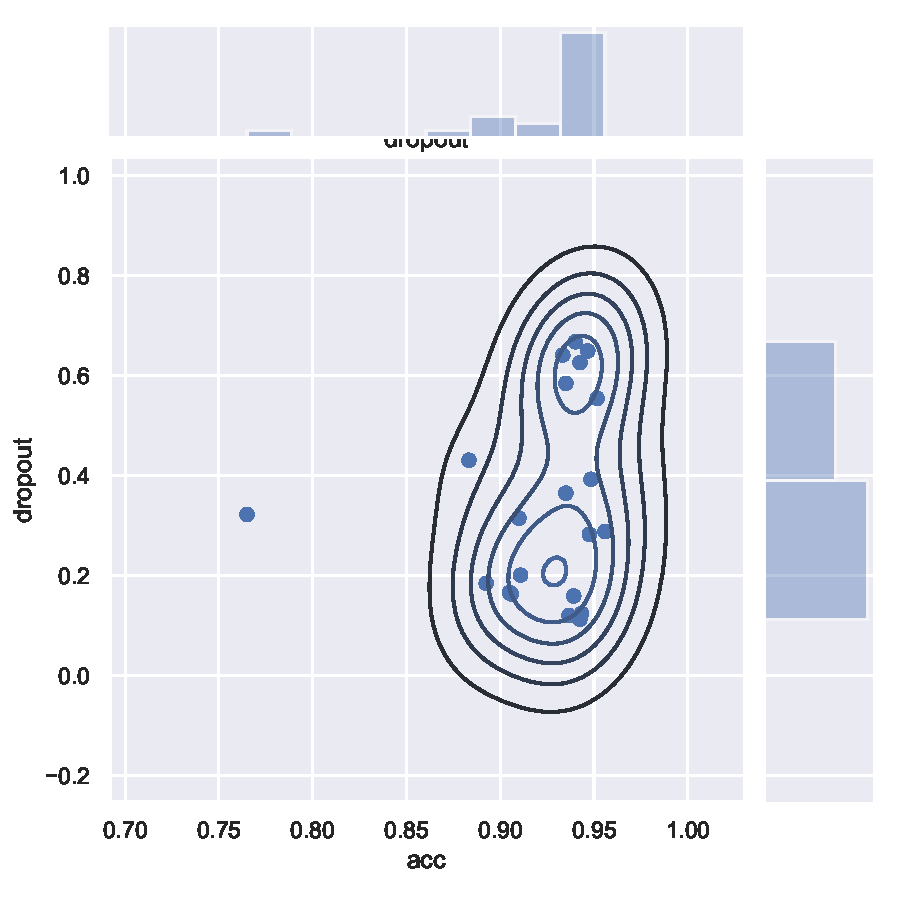
\includegraphics[scale=0.5]{anhang/GA_50_mnist_digits_True_small_jointplot_dropout.pdf}
  \caption{Dichte-Diagramm des Dropouts in Verbindung mit der Klassifizierungsgenauigkeit(acc)}
  
\end{figure}

\begin{figure}[H]
  \centering  
  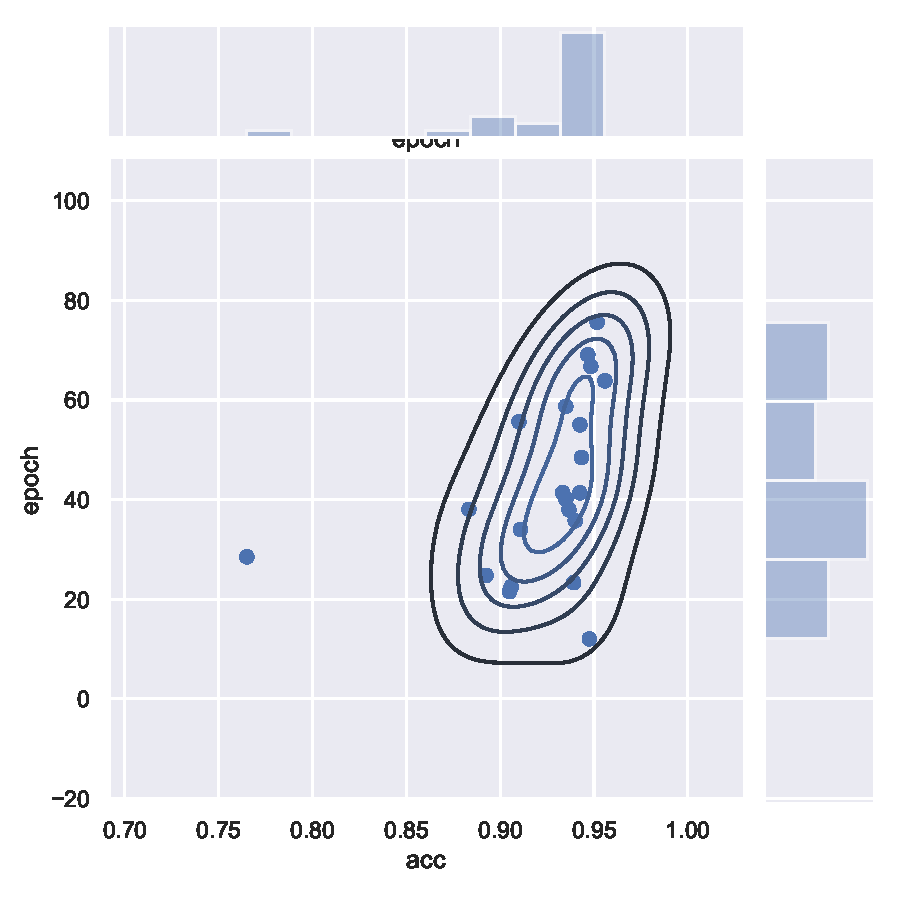
\includegraphics[scale=0.5]{anhang/GA_50_mnist_digits_True_small_jointplot_epoch.pdf}
  \caption{Dichte-Diagramm der Epochenanzahl in Verbindung mit der Klassifizierungsgenauigkeit(acc)}
  
\end{figure}

\begin{figure}[H]
  \centering  
  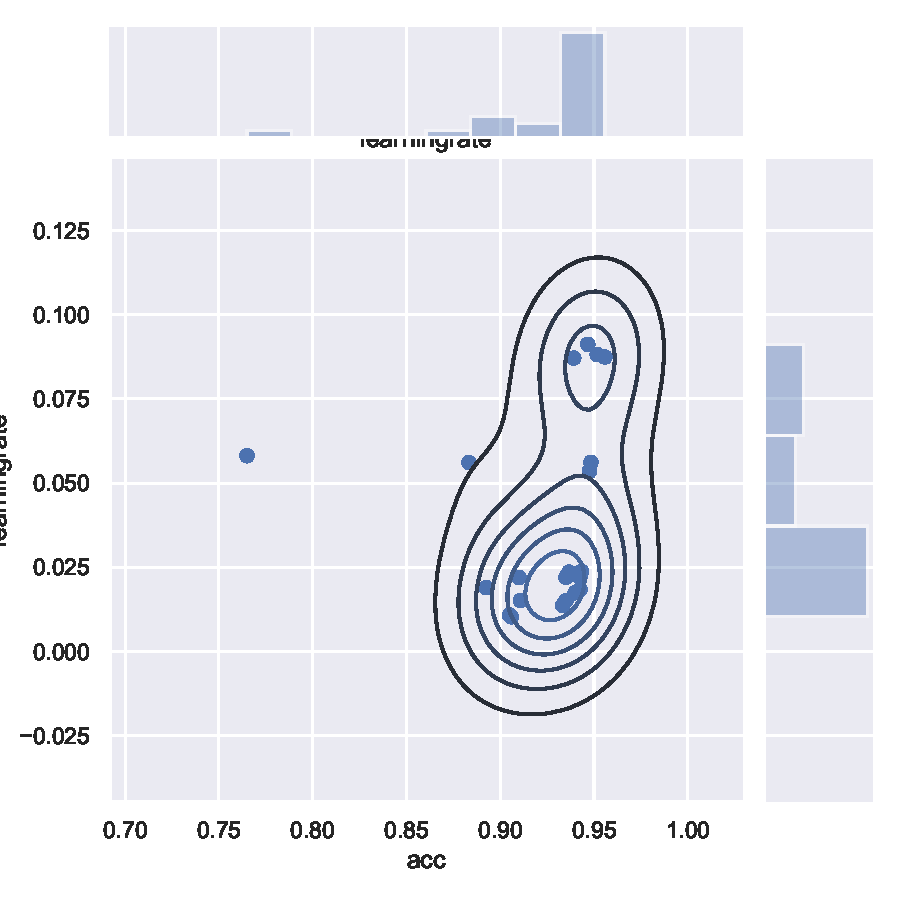
\includegraphics[scale=0.5]{anhang/GA_50_mnist_digits_True_small_jointplot_learningrate.pdf}
  \caption{Dichte-Diagramm der Lernrate in Verbindung mit der Klassifizierungsgenauigkeit(acc)}
  
\end{figure}

\begin{figure}[H]
  \centering  
  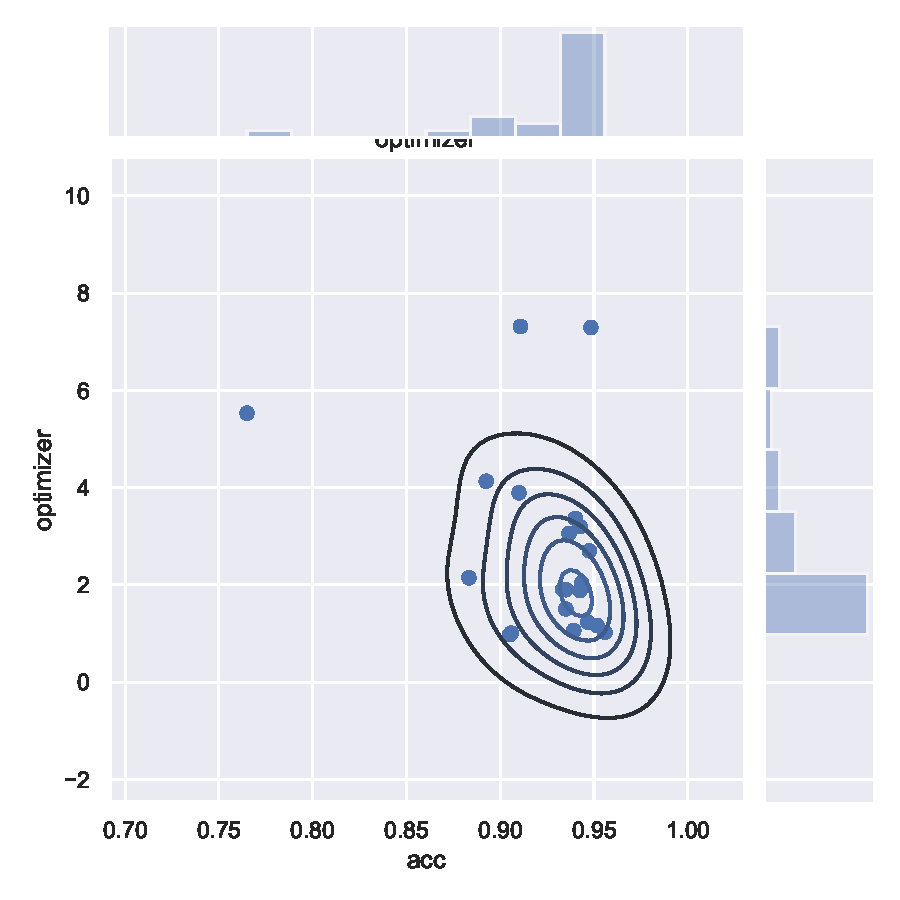
\includegraphics[scale=0.5]{anhang/GA_50_mnist_digits_True_small_jointplot_optimizer.pdf}
  \caption{Dichte-Diagramm der Optimierer in Verbindung mit der Klassifizierungsgenauigkeit(acc)}
  
\end{figure}

\subsection{50 Iterationen des Genetischen Algorithmus des großen Fully-Connected Netzes}
\begin{figure}[H]
  \centering  
  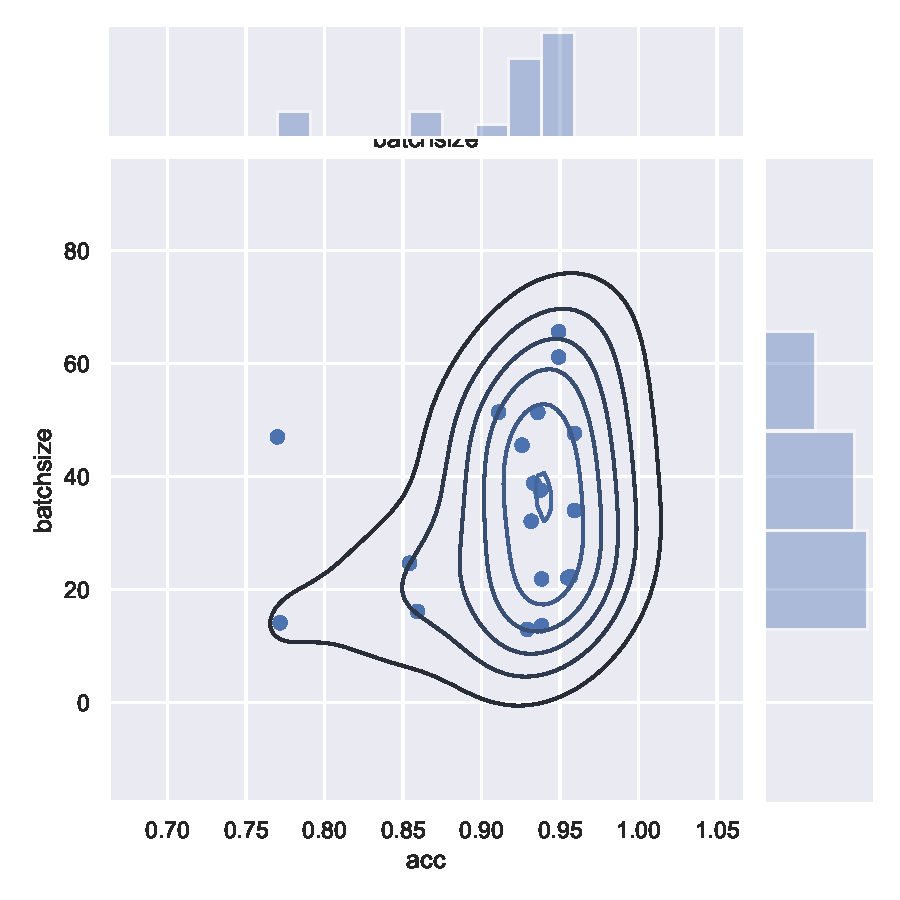
\includegraphics[scale=0.5]{anhang/GA_50_mnist_digits_True_big_jointplot_batchsize.pdf}
  \caption{Dichte-Diagramm der Batchsize in Verbindung mit der Klassifizierungsgenauigkeit(acc)}
  
\end{figure}

\begin{figure}[H]
  \centering  
  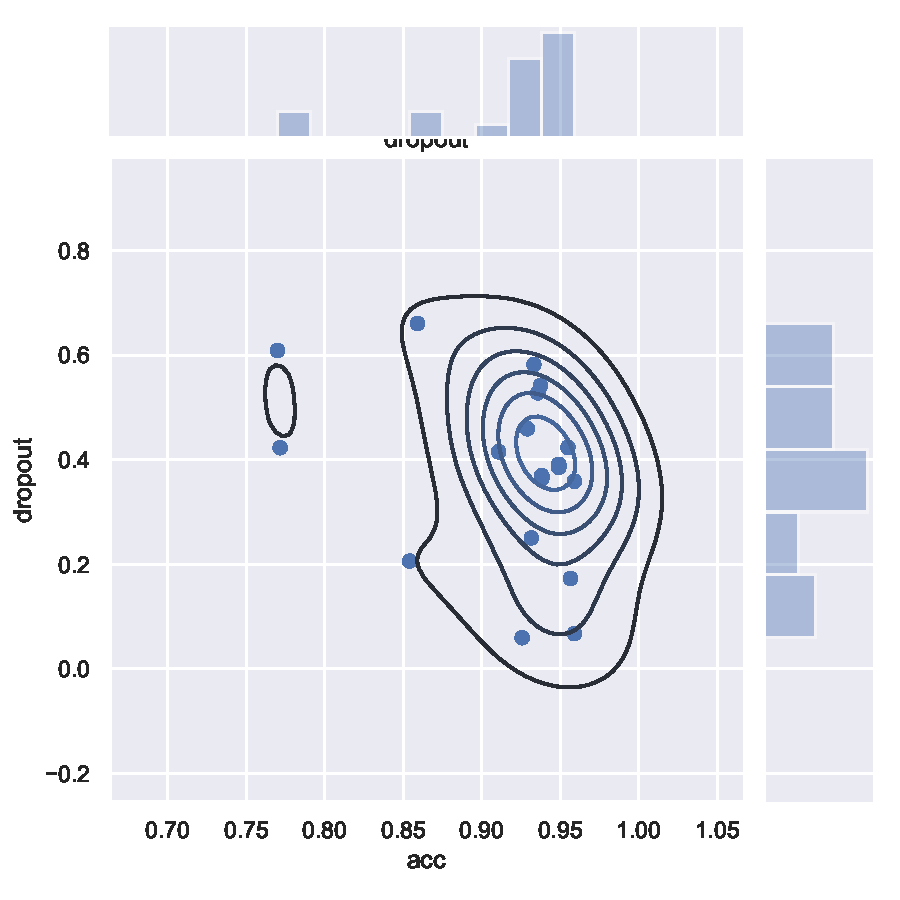
\includegraphics[scale=0.5]{anhang/GA_50_mnist_digits_True_big_jointplot_dropout.pdf}
  \caption{Dichte-Diagramm des Dropouts in Verbindung mit der Klassifizierungsgenauigkeit(acc)}
  
\end{figure}

\begin{figure}[H]
  \centering  
  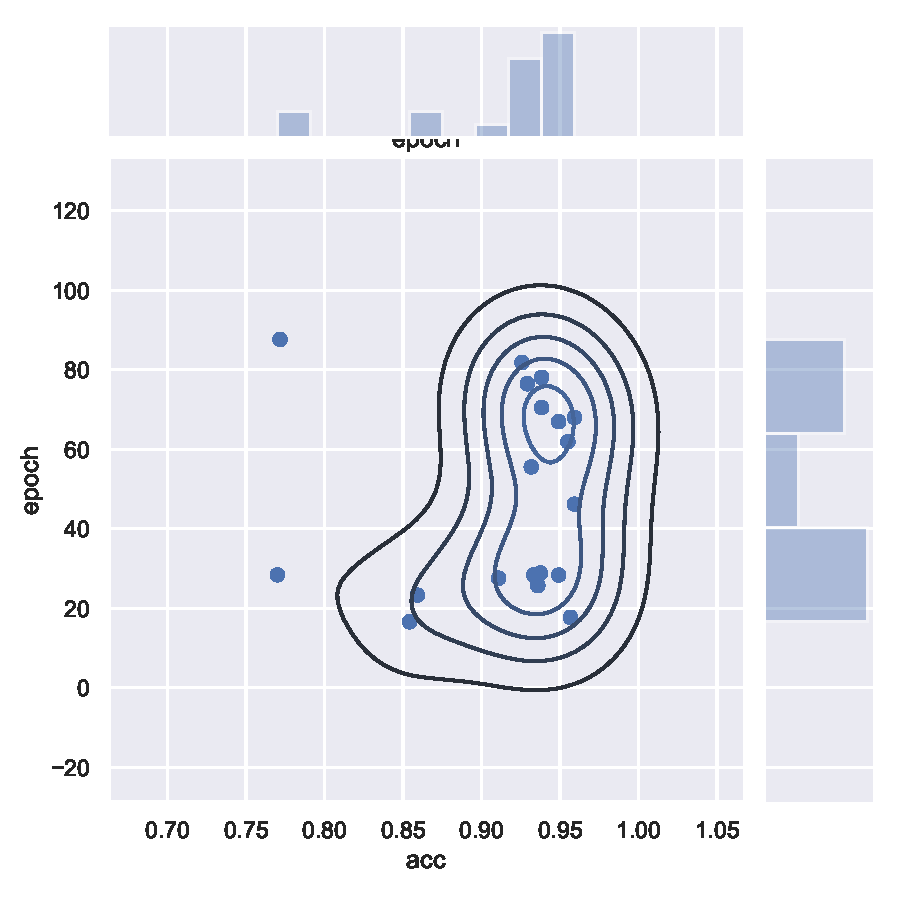
\includegraphics[scale=0.5]{anhang/GA_50_mnist_digits_True_big_jointplot_epoch.pdf}
  \caption{Dichte-Diagramm der Epochenanzahl in Verbindung mit der Klassifizierungsgenauigkeit(acc)}
\end{figure}

\begin{figure}[H]
  \centering  
  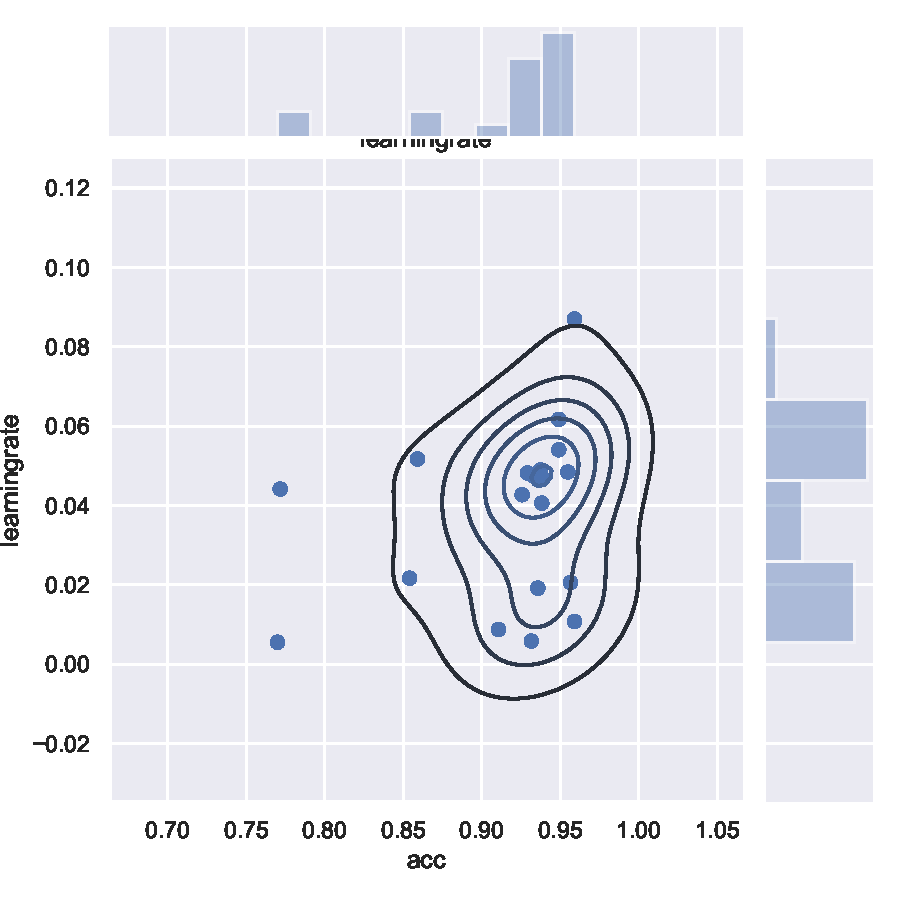
\includegraphics[scale=0.5]{anhang/GA_50_mnist_digits_True_big_jointplot_learningrate.pdf}
  \caption{Dichte-Diagramm der Lernrate in Verbindung mit der Klassifizierungsgenauigkeit(acc)}
  
\end{figure}

\begin{figure}[H]
  \centering  
  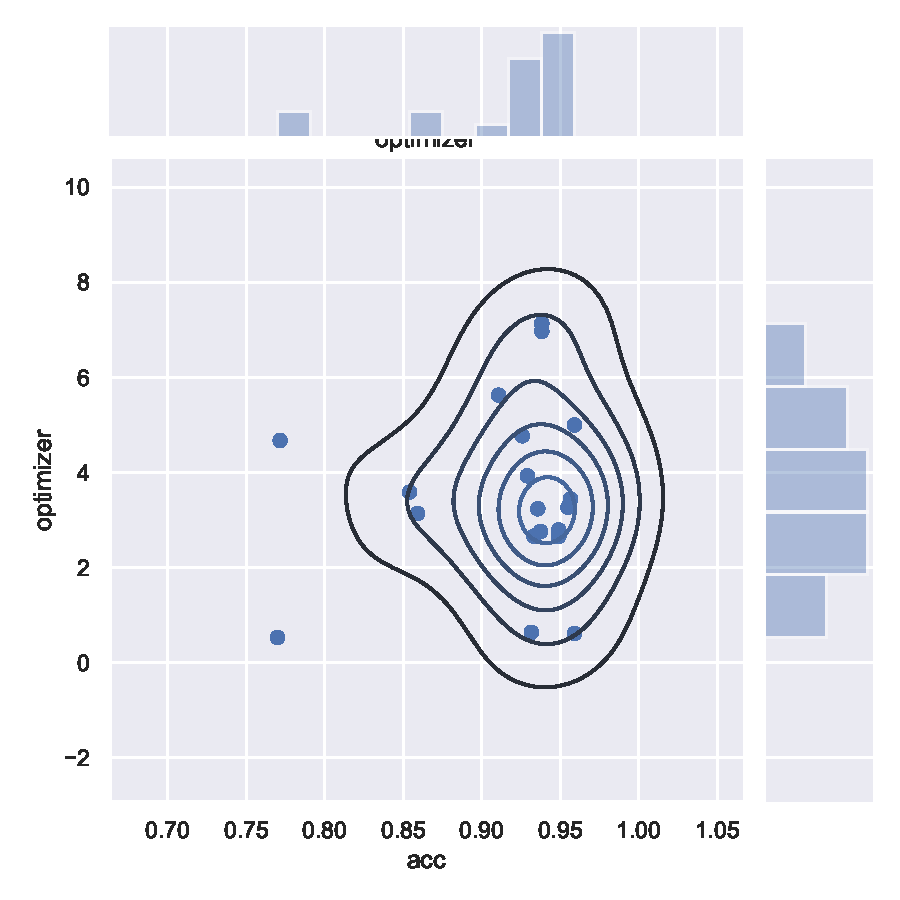
\includegraphics[scale=0.5]{anhang/GA_50_mnist_digits_True_big_jointplot_optimizer.pdf}
  \caption{Dichte-Diagramm der Optimierer in Verbindung mit der Klassifizierungsgenauigkeit(acc)}
  
\end{figure}

\subsection{250 Iterationen des Genetischen Algorithmus des kleinen Fully-Connected Netzes}
\begin{figure}[H]
  \centering  
  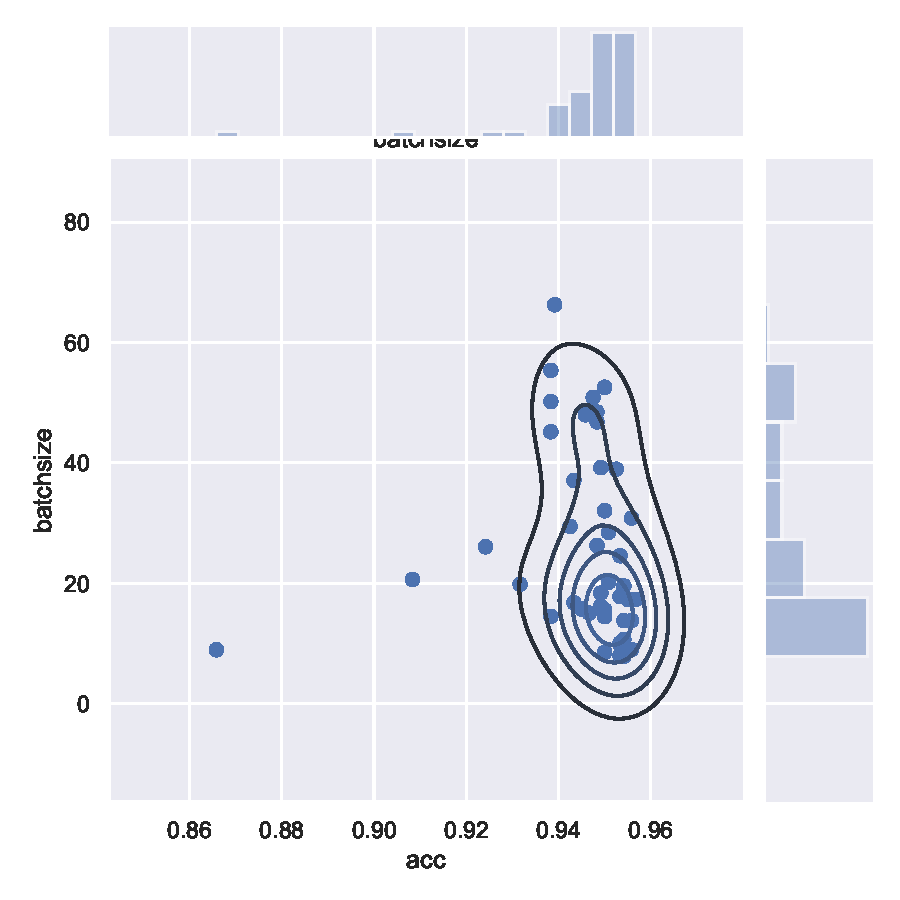
\includegraphics[scale=0.5]{anhang/GA_250_mnist_digits_True_small_jointplot_batchsize.pdf}
  \caption{Dichte-Diagramm der Batchsize in Verbindung mit der Klassifizierungsgenauigkeit(acc)}
  
\end{figure}

\begin{figure}[H]
  \centering  
  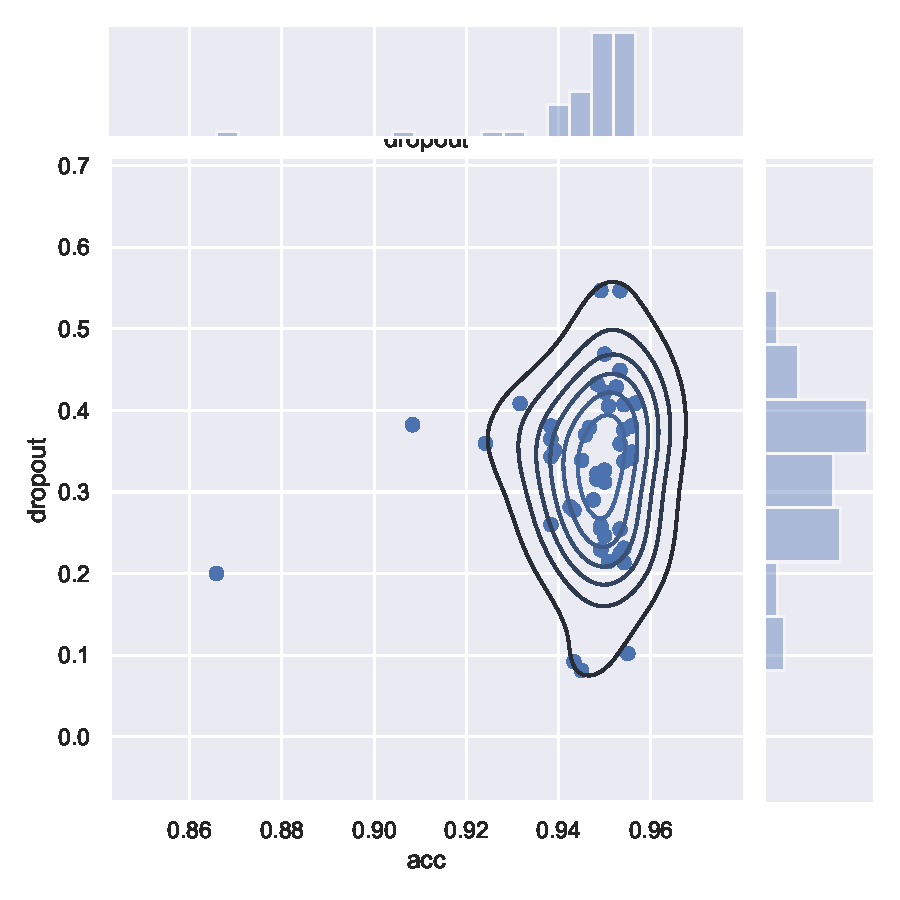
\includegraphics[scale=0.5]{anhang/GA_250_mnist_digits_True_small_jointplot_dropout.pdf}
  \caption{Dichte-Diagramm des Dropouts in Verbindung mit der Klassifizierungsgenauigkeit(acc)}
  
\end{figure}

\begin{figure}[H]
  \centering  
  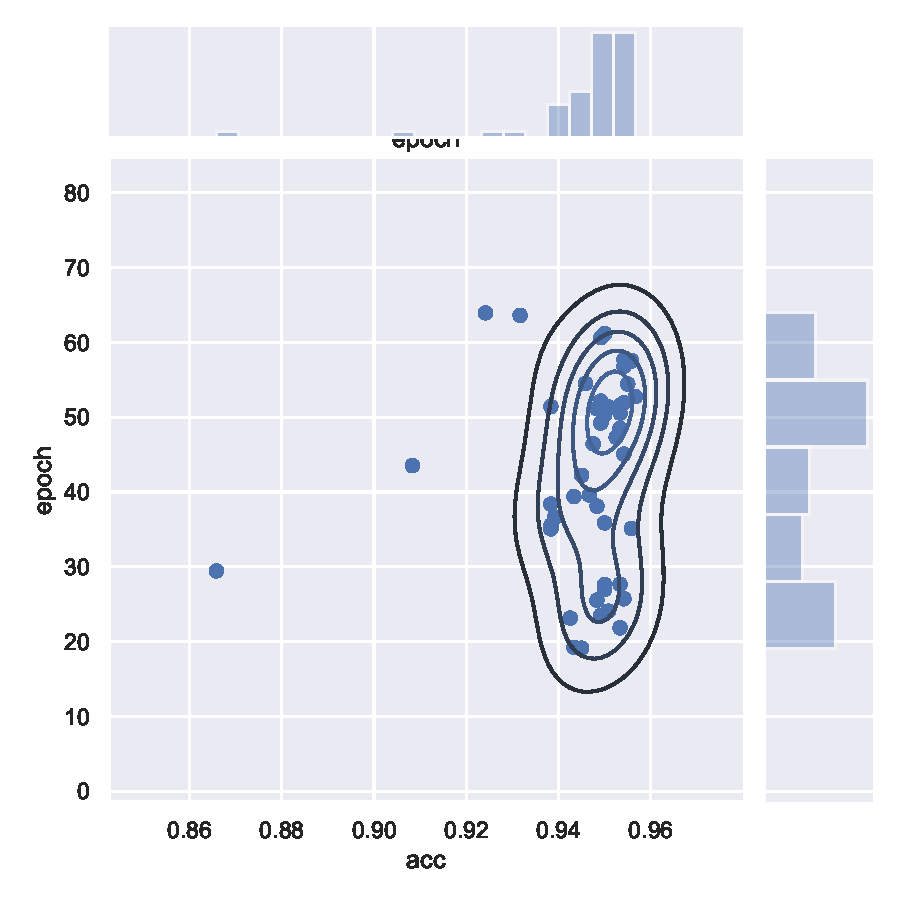
\includegraphics[scale=0.5]{anhang/GA_250_mnist_digits_True_small_jointplot_epoch.pdf}
  \caption{Dichte-Diagramm der Epochenanzahl in Verbindung mit der Klassifizierungsgenauigkeit(acc)}
  
\end{figure}

\begin{figure}[H]
  \centering  
  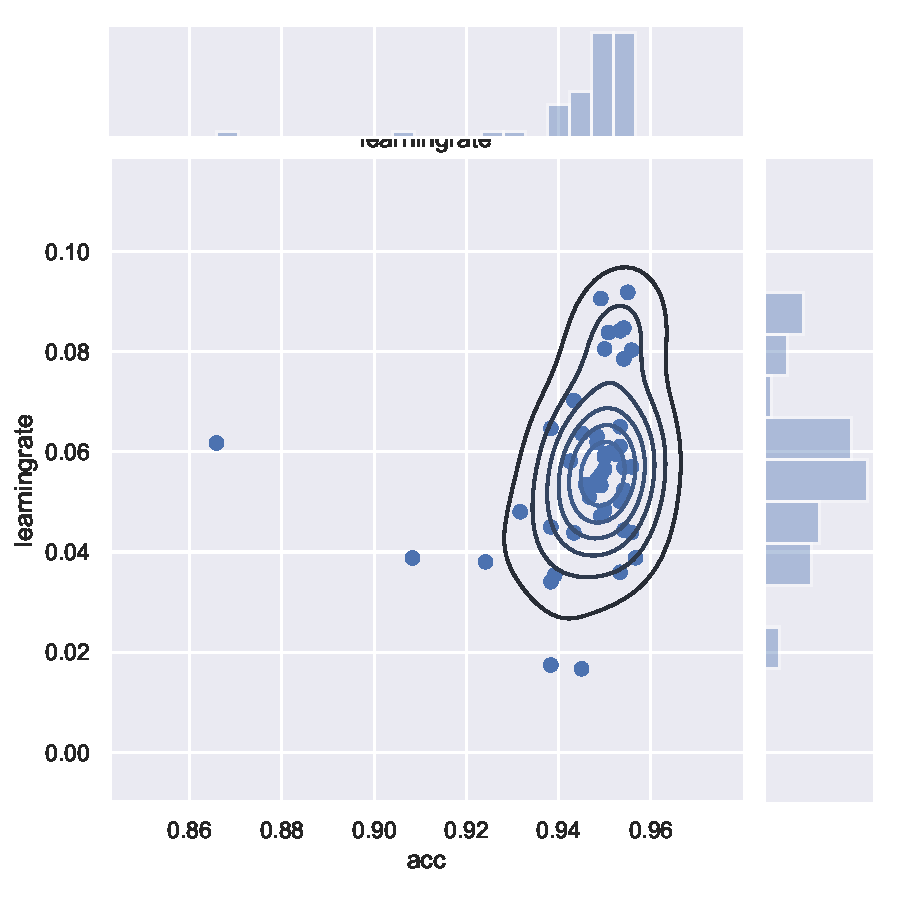
\includegraphics[scale=0.5]{anhang/GA_250_mnist_digits_True_small_jointplot_learningrate.pdf}
  \caption{Dichte-Diagramm der Lernrate in Verbindung mit der Klassifizierungsgenauigkeit(acc)}
  
\end{figure}

\begin{figure}[H]
  \centering  
  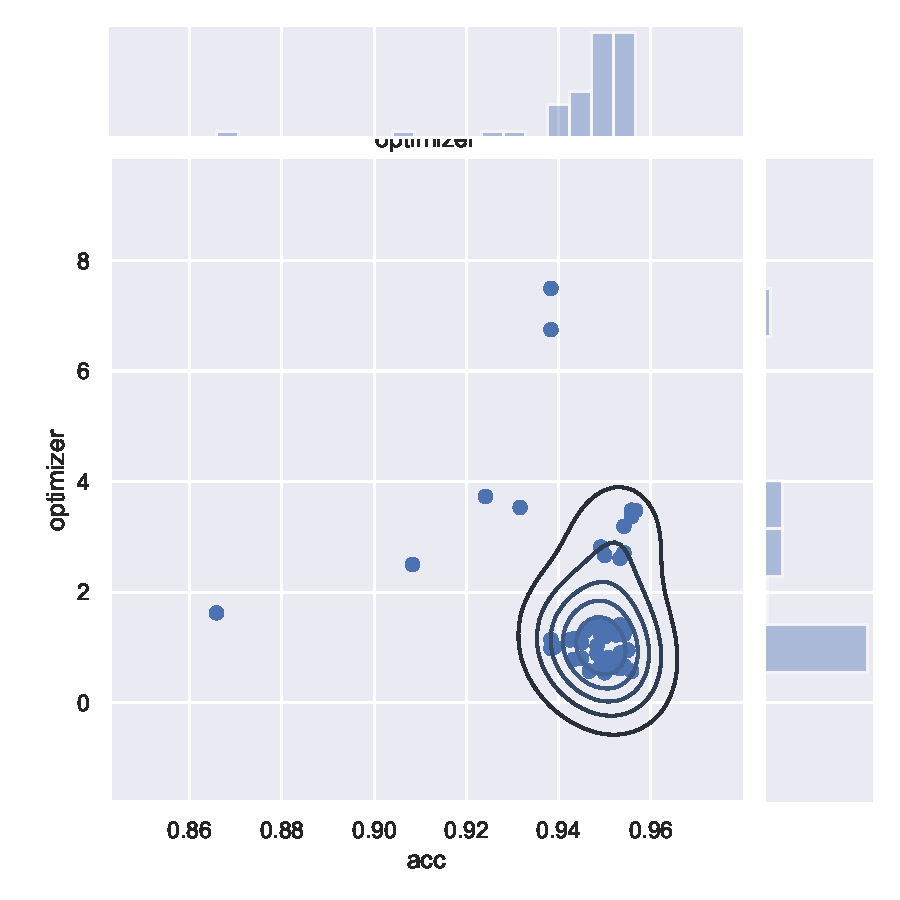
\includegraphics[scale=0.5]{anhang/GA_250_mnist_digits_True_small_jointplot_optimizer.pdf}
  \caption{Dichte-Diagramm der Optimierer in Verbindung mit der Klassifizierungsgenauigkeit(acc)}
  
\end{figure}


\subsection{250 Iterationen des Genetischen Algorithmus des großen Fully-Connected Netzes}
\begin{figure}[H]
  \centering  
  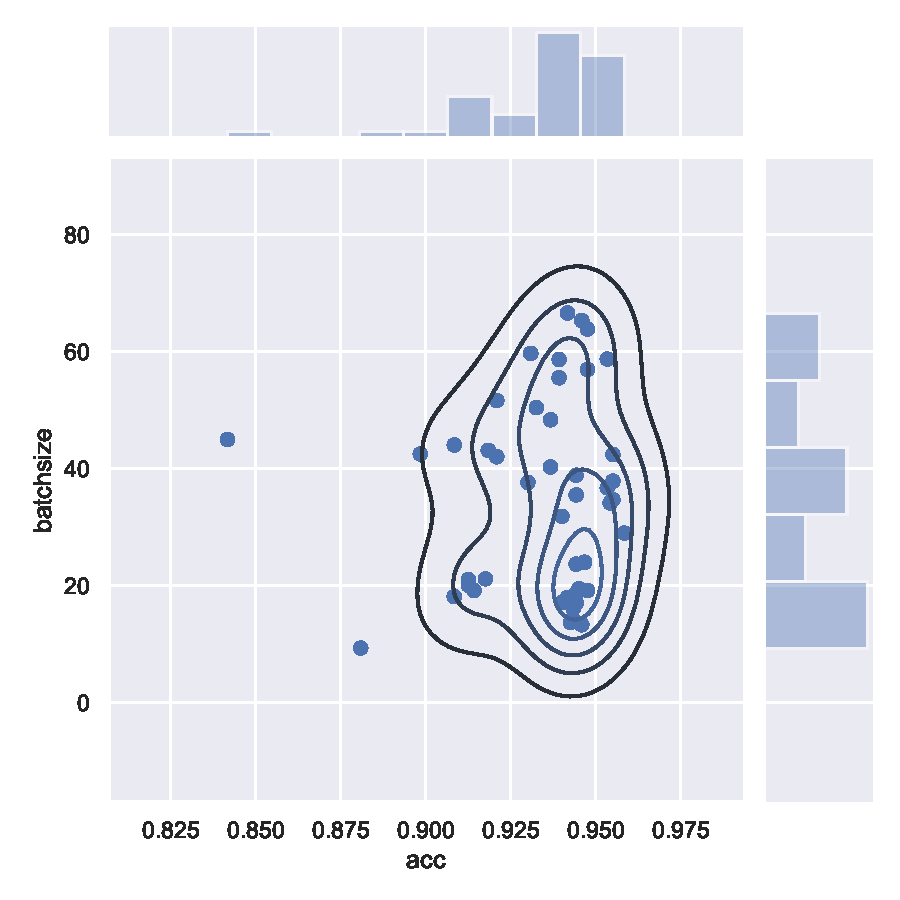
\includegraphics[scale=0.5]{anhang/GA_250_mnist_digits_True_big_jointplot_batchsize.pdf}
  \caption{Dichte-Diagramm der Batchsize in Verbindung mit der Klassifizierungsgenauigkeit(acc)}
  
\end{figure}

\begin{figure}[H]
  \centering  
  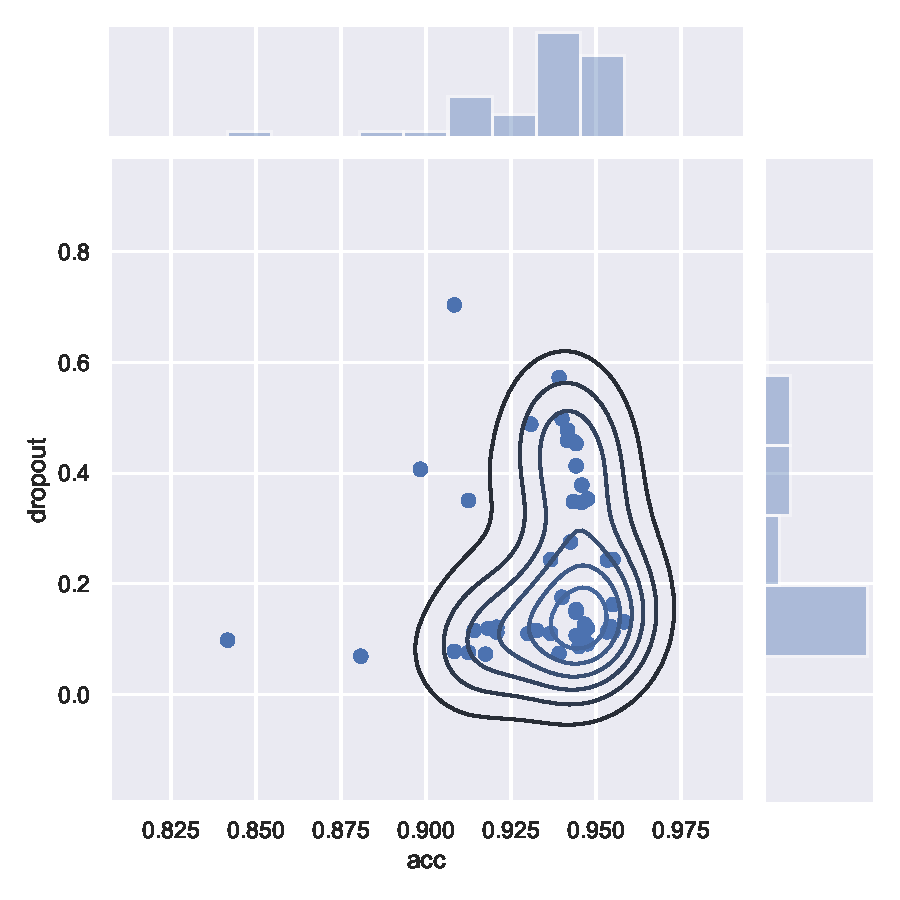
\includegraphics[scale=0.5]{anhang/GA_250_mnist_digits_True_big_jointplot_dropout.pdf}
  \caption{Dichte-Diagramm des Dropouts in Verbindung mit der Klassifizierungsgenauigkeit(acc)}
  
\end{figure}

\begin{figure}[H]
  \centering  
  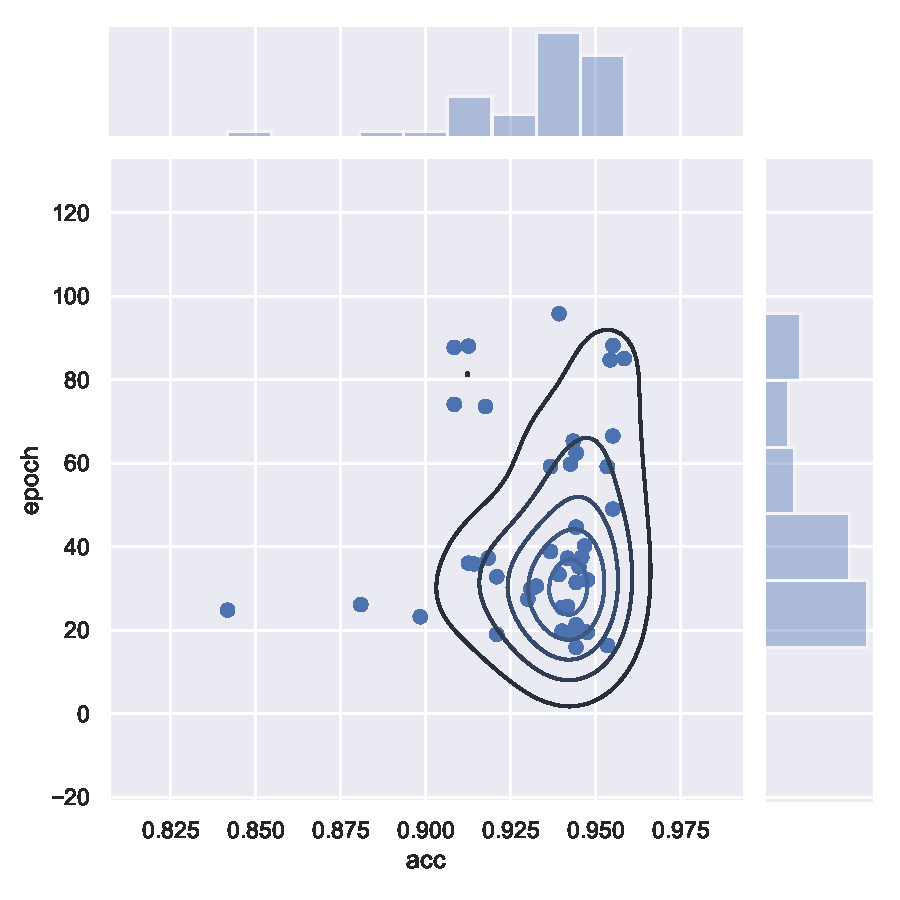
\includegraphics[scale=0.5]{anhang/GA_250_mnist_digits_True_big_jointplot_epoch.pdf}
  \caption{Dichte-Diagramm der Epochenanzahl in Verbindung mit der Klassifizierungsgenauigkeit(acc)}
  
\end{figure}

\begin{figure}[H]
  \centering  
  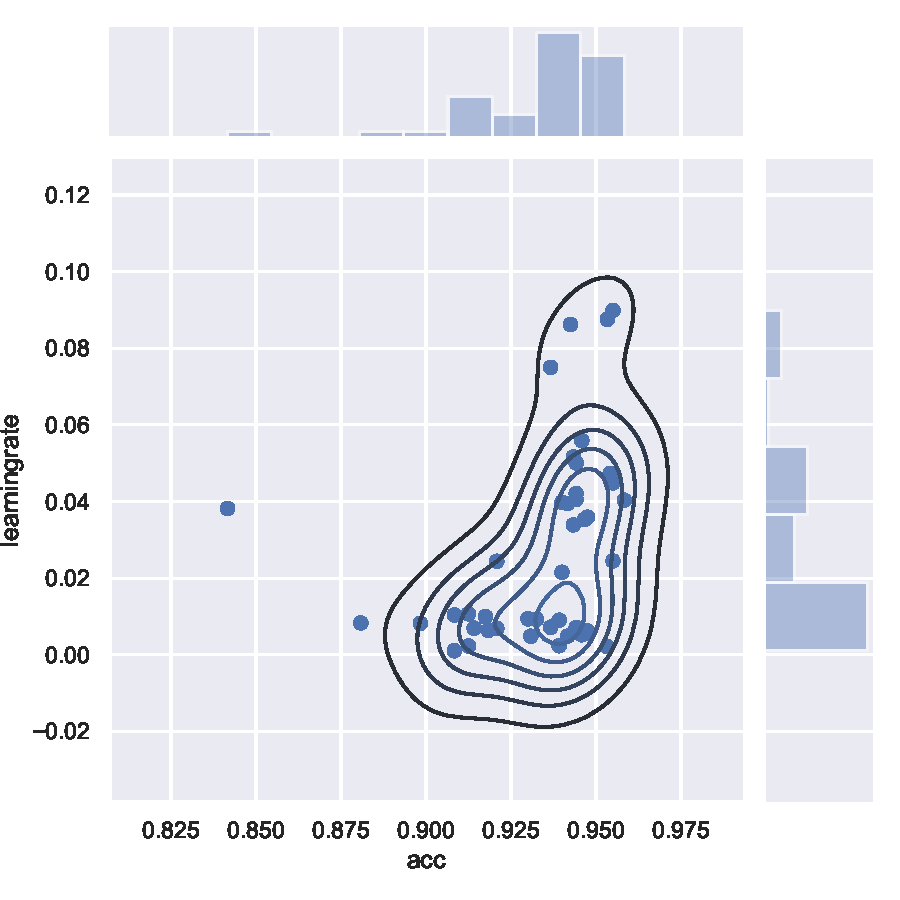
\includegraphics[scale=0.5]{anhang/GA_250_mnist_digits_True_big_jointplot_learningrate.pdf}
  \caption{Dichte-Diagramm der Lernrate in Verbindung mit der Klassifizierungsgenauigkeit(acc)}
  
\end{figure}

\begin{figure}[H]
  \centering  
  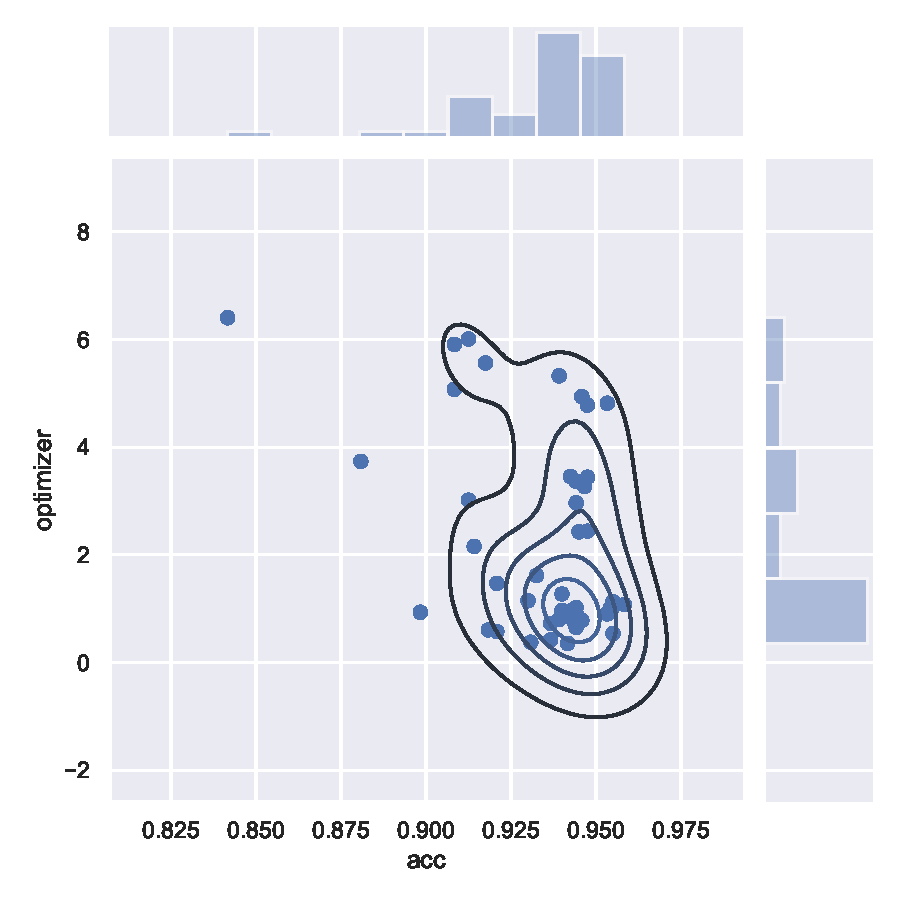
\includegraphics[scale=0.5]{anhang/GA_250_mnist_digits_True_big_jointplot_optimizer.pdf}
  \caption{Dichte-Diagramm der Optimierer in Verbindung mit der Klassifizierungsgenauigkeit(acc)}
  
\end{figure}

\subsection{50 Iterationen des Genetischen Algorithmus des Convolutional Neural Network}
\begin{figure}[H]
  \centering  
  \includegraphics[scale=0.5]{anhang/GA_50_cifar10_True_big_jointplot_batchsize.pdf}
  \caption{Dichte-Diagramm der Batchsize in Verbindung mit der Klassifizierungsgenauigkeit(acc)}
  
\end{figure}

\begin{figure}[H]
  \centering  
  \includegraphics[scale=0.5]{anhang/GA_50_cifar10_True_big_jointplot_dropout.pdf}
  \caption{Dichte-Diagramm des Dropouts in Verbindung mit der Klassifizierungsgenauigkeit(acc)}
  
\end{figure}

\begin{figure}[H]
  \centering  
  \includegraphics[scale=0.5]{anhang/GA_50_cifar10_True_big_jointplot_epoch.pdf}
  \caption{Dichte-Diagramm der Epochenanzahl in Verbindung mit der Klassifizierungsgenauigkeit(acc)}
  
\end{figure}

\begin{figure}[H]
  \centering  
  \includegraphics[scale=0.5]{anhang/GA_50_cifar10_True_big_jointplot_learningrate.pdf}
  \caption{Dichte-Diagramm der Lernrate in Verbindung mit der Klassifizierungsgenauigkeit(acc)}
  
\end{figure}

\begin{figure}[H]
  \centering  
  \includegraphics[scale=0.5]{anhang/GA_50_cifar10_True_big_jointplot_optimizer.pdf}
  \caption{Dichte-Diagramm des Optimierers in Verbindung mit der Klassifizierungsgenauigkeit(acc)}
  
\end{figure}

\subsection{250 Iterationen des Genetischen Algorithmus des Convolutional Neural Network}
\begin{figure}[H]
  \centering  
  \includegraphics[scale=0.5]{anhang/GA_250_cifar10_True_big_jointplot_batchsize.pdf}
  \caption{Dichte-Diagramm der Batchsize in Verbindung mit der Klassifizierungsgenauigkeit(acc)}
  
\end{figure}

\begin{figure}[H]
  \centering  
  \includegraphics[scale=0.5]{anhang/GA_250_cifar10_True_big_jointplot_dropout.pdf}
  \caption{Dichte-Diagramm des Dropouts in Verbindung mit der Klassifizierungsgenauigkeit(acc)}
  
\end{figure}

\begin{figure}[H]
  \centering  
  \includegraphics[scale=0.5]{anhang/GA_250_cifar10_True_big_jointplot_epoch.pdf}
  \caption{Dichte-Diagramm der Epochenanzahl in Verbindung mit der Klassifizierungsgenauigkeit(acc)}
  
\end{figure}

\begin{figure}[H]
  \centering  
  \includegraphics[scale=0.5]{anhang/GA_250_cifar10_True_big_jointplot_learningrate.pdf}
  \caption{Dichte-Diagramm der Lernrate in Verbindung mit der Klassifizierungsgenauigkeit(acc)}
  
\end{figure}

\begin{figure}[H]
  \centering  
  \includegraphics[scale=0.5]{anhang/GA_250_cifar10_True_big_jointplot_optimizer.pdf}
  \caption{Dichte-Diagramm des Optimierers in Verbindung mit der Klassifizierungsgenauigkeit(acc)}
  
\end{figure}